\documentclass[11pt,aspectratio=1610]{beamer}
\usepackage[utf8]{inputenc} % Modifier selon l'encodage (latin1, utf8...)
%% Ajouter tous \usepackage{}s utiles, par exemple :
\usepackage[T1]{fontenc}
\usepackage[french]{babel}
\usepackage{calligra}

\mode<presentation>
\usetheme{tptnew}%[authorintitle,bodyframecount,bgblocks foreground,nohelvet]{tptnew}
\usepackage{bera}

% https://tex.stackexchange.com/questions/3676/too-many-math-alphabets-error
\newcommand\hmmax{0}
\newcommand\bmmax{0}

\usepackage{amsmath}			% Permet de taper des formules mathématiques
\usepackage{amssymb}			% Permet d'utiliser des symboles mathématiques
\usepackage{amsfonts}			% Permet d'utiliser des polices mathématiques
\usepackage{amsthm}				% Permet d'écrire des théorèmes
\usepackage{nicefrac}			% Fractions 'inline'
\usepackage{stmaryrd}			% Pour les brackets
\usepackage{mathtools}			% Pour la KL div
\usepackage{bm}                 % Pour les vecteurs en gras
\usepackage{bbm}

\usepackage{graphicx}
\usepackage{caption}

\usepackage{ragged2e} % For justifying text

\usepackage{multicol}

\usepackage{tikz}
\tikzstyle{arrow}=[draw, -latex]
\usetikzlibrary{shapes,arrows}
\usetikzlibrary{positioning,fit,calc}
\tikzstyle{block} = [draw, fill=white, rectangle, 
minimum height=3em, minimum width=6em]
\tikzstyle{input} = [coordinate]
\tikzstyle{output} = [coordinate]
\tikzstyle{arrow}=[draw, -latex]

\usepackage{pifont} % For symbols, icônes...
\usepackage{xcolor}
\newcommand{\fancybullet}{\ding{51}}
\newcommand{\boxqmark}{\fbox{\textbf{?}}}

\usepackage[utf8]{inputenc}

\def\BibTeX{{\rm B\kern-.05em{\sc i\kern-.025em b}\kern-.08em
 T\kern-.1667em\lower.7ex\hbox{E}\kern-.125emX}}

\DeclareMathOperator*{\argmin}{argmin}
\DeclareMathOperator*{\argmax}{argmax}

\newtheorem{conjecture}{Conjecture}

%% Faire apparaître le plan avant chaque section :
%\AtBeginSection[]{\contentsframe[currentsection]}
%\renewcommand*\contentsframename{Outline}


%----------------------------------------------------------------------------------------
%	TITLE PAGE
%----------------------------------------------------------------------------------------


\title{\color{purple}Low-overhead ML methods for beamforming/combining in RIS assisted millimeter-wave massive MIMO systems} 
\author{Oumaïma Bounhar}
\institute{\normalsize Supervised by Pr. \textbf{Ghaya Rekaya-Ben Othman} \\[4pt]
\textbf{Télécom Paris, Institut-Mines-Télécom}, Palaiseau, France \\[6pt]
\raisebox{4mm}{\href{https://www.telecom-paris.fr/en/home}{
\includegraphics[height=12mm]{Figures/tp.pdf}}}}
\date{\today}

\let\emph\alert
\newcommand\alertb[1]{\textcolor{blue}{#1}}

\newcommand{\E}{\ensuremath\mathbb{E}}
\renewcommand{\P}{\ensuremath\mathbb{P}}
\renewcommand{\d}{\ensuremath\,\mathrm{d}}
\newcommand{\dx}{\ensuremath\,\mathrm{d}x}
\newcommand{\dt}{\ensuremath\,\mathrm{d}t}

\let\leq\leqslant
\let\geq\geqslant
\let\eps\varepsilon
\let\phi\varphi

\def\sumint{\mathchoice{\xsumint\displaystyle\textstyle\sum}%
	{\xsumint\textstyle\scriptstyle\Sigma}%
	{\xsumint\scriptstyle\scriptstyle\Sigma}%
	{\xsumint\scriptscriptstyle\scriptscriptstyle\Sigma}%
	\!\int}
\def\xsumint#1#2#3{{\setbox0=\hbox{${#2#3}{#1\int}$}
		\vcenter{\hbox{$#2#3$}}\kern-.5\wd0}}

\usepackage{array}
\usepackage{dutchcal}

\usepackage{graphicx}
\graphicspath{{.}{img/}{logo/}{../figs/}{Figures/}}
\DeclareGraphicsExtensions{.pdf,.png,.jpg}

%\input{../../note_mi/CommandesPerso}

\usepackage{wrapfig}                   
\usepackage{subcaption}
% \usepackage{pdfpages}
% \usepackage{rotating}
\usepackage{pgfplots}
\usepgfplotslibrary{groupplots,dateplot}
\usepackage{tikz}
\usetikzlibrary{backgrounds,automata,arrows,shadows,positioning, shapes}
\usetikzlibrary{decorations.pathreplacing,angles,quotes}
\pgfplotsset{width=7cm,compat=1.3}
\usepackage{import}

\usepackage{pgfkeys}
\newenvironment{customlegend}[1][]{%
	\begingroup
	\csname pgfplots@init@cleared@structures\endcsname
	\pgfplotsset{#1}%
}{%
	\csname pgfplots@createlegend\endcsname
	\endgroup
}%
\def\addlegendimage{\csname pgfplots@addlegendimage\endcsname}

\definecolor{antiquewhite254229217}{RGB}{254,229,217}
\definecolor{darkgray176}{RGB}{176,176,176}
\definecolor{firebrick2032429}{RGB}{203,24,29}
\definecolor{gainsboro229}{RGB}{229,229,229}
\definecolor{lightsalmon252174145}{RGB}{252,174,145}
\definecolor{lightsalmon252146114}{RGB}{252,146,114}
\definecolor{tomato25110674}{RGB}{251,106,74}
\definecolor{darkseagreen116196118}{RGB}{116,196,118}
\definecolor{lightgreen161217155}{RGB}{161,217,155}
\definecolor{lightgray204}{RGB}{204,204,204}

\newcommand\Fontvi{\fontsize{9}{9.5}\selectfont}

\begin{document}

    \begin{frame}
        \titlepage  
    \end{frame}

    %----------------------------------------------------------------------------------------
    %	PRESENTATION SLIDES
    %----------------------------------------------------------------------------------------
    
    % \begin{frame}
    %     \frametitle{Thesis Advancement \& Context}
    %     \begin{tikzpicture}[>=stealth, thick]

    %         % Draw main line
    %         \draw[->] (0,0) -- (12,0);

    %         % Year markers
    %         \foreach \x/\year in {0/Start,4/Year 1,8/Year 2,12/Year 3} {
    %             \draw (\x,0.15) -- (\x,-0.15); % tick
    %             \node[above=4pt] at (\x,0.15) {\textbf{\year}};
    %         }

    %         % Current position
    %         \draw[red, thick] (3,0.4) -- (3,-0.5); % vertical line
    %         \node[below=14pt, text=red] at (3,-0.2) {I am here};

    %         % Optional text underneath timeline
    %         \node[below=28pt, align=center] at (3,-0.6)
    %             {\shortstack[l]{$\bullet$ 1st CSI \\ $\bullet$ PEPR 5G YACARI Project}};
    %     \end{tikzpicture}
    % \end{frame}

    \begin{frame}
        \frametitle{Thesis Advancement \& Context}
        \begin{tikzpicture}[>=stealth, thick]

            % Main line
            \draw[->] (0,0) -- (12,0);

            % Year markers
            \foreach \x/\year in {0/Jan. 2025,4/Year 1,8/Year 2,12/Year 3} {
                \draw (\x,0.15) -- (\x,-0.15);
                \node[above=4pt] at (\x,0.15) {\textbf{\year}};
            }

            % Current position (3 months left in Year 2, i.e. 1 unit before the Year 2 mark)
            \draw[red, thick] (7.0,0.3) -- (7.0,-0.6);
            \node[below=14pt, text=red] at (7.0,-0.4) {I am here};

            % % Current tasks
            % \node[below=38pt, align=center] at (3,-0.8)
            %     {\shortstack[l]{$\bullet$ 1st CSI \\ $\bullet$ PEPR 5G YACARI Project}};

            % Left double-headed arrow (past work)
            \draw[blue, <->, thick] (0.2,-0.4) -- (6.9,-0.4);
            \node[below=4pt, text=blue] at (3.5,-0.4) {Past work};

            % Right double-headed arrow (future work)
            \draw[blue, <->, thick] (7.1,-0.4) -- (11.8,-0.4);
            \node[below=4pt, text=blue] at (9.5,-0.4) {Future work};

        \end{tikzpicture}
    \end{frame}

    %------------------------------------------------

    \begin{frame}
        \frametitle{Outline}
        \tableofcontents
    \end{frame}

    %------------------------------------------------

    \section{Context}

    %------------------------------------------------

    % \begin{frame}
    %     \frametitle{Context}
    %     \begin{itemize}[<+->]
    %         \item 5G \& 6G rely on Milimiter waves (mmWaves) for higher data rates;
    %         \item mmWaves suffer from fading environments;
    %         \item RIS is a promising solution with low power consumption.
    %     \end{itemize}
    % \end{frame}

    \begin{frame}
        \frametitle{Context}
        \begin{columns}[T] % T aligns the top of both columns
            % Left column
            \begin{column}{0.5\textwidth}
                \includegraphics<1-4>[width=\textwidth]{Figures/PassiveRIS.png}
            \end{column}

            % Right column
            \begin{column}{0.49\textwidth}
                \begin{itemize}
                    \item<2-|alert@2> mmWaves suffer from fading environments; 
                    \item<3-|alert@3> 5G \& 6G rely on millimeter waves (mmWaves) for higher coverage;
                    \item<4-|alert@4> RIS is a promising solution with low power consumption.
                \end{itemize}
            \end{column}
        \end{columns}
    \end{frame}

    %------------------------------------------------

    \section{System Model}

    %------------------------------------------------

    %------------------------------------------------
    % Part that needs a change, inctroduce the figure "No_direct_link.png" at slide 5 of this frame
    %------------------------------------------------

    \begin{frame}
        \frametitle{System Model}
        \begin{columns}[T] % T aligns the top of both columns
            \begin{column}{0.5\textwidth}
                \includegraphics<1-4>[width =\textwidth]{Figures/System_setup.png}
                \includegraphics<5-6>[width =\textwidth]{Figures/No_direct_link.png}
            \end{column}    
            \onslide <1-6>
            \begin{column}{0.49\textwidth}
                % \begin{itemize} <+-> % By default dispalys items one after the other.
                % \begin{itemize} <+> % By default dispalys items one after the other by removes all the otheR ones.
                \begin{itemize} [<+-|alert@+>] % By default dispalys items one after the other.
                % \begin{itemize}
                    \item $\mathrm N_{\text{UE}} = 1$;
                    \item $\mathrm N_{\text{BS}} = 64$;
                    \item $\mathrm N_{\text{RIS}} = 100$;
                    \item The direct link is blocked.
                \end{itemize}
                \onslide <5-6> We consider half-wave spaced ULAs:
                \vspace{-6mm} \\
                \begin{equation*}
                    \begin{split}   
                        \bold{H}_{\text{BS}} &=  \mathbf{a}_{\mathrm N}(\Phi_{1}) \mathbf{a}_{\mathrm M}^{H}(\Phi_{2}) \\
                        \bold{h}_{\text{UE}} &=  \mathbf{a}_{1}(\Phi_{3}) \mathbf{a}_{\mathrm N}^{H}(\Phi_{4}) 
                    \end{split}
                \end{equation*}
                \onslide <6> where the steering vector is: 
                \vspace{-3mm}
                \begin{equation*}
                    \mathbf{a}_{\mathrm N}(\Phi) = [1,e^{j\pi \sin (\Phi)},\ldots, e^{j\pi (\mathrm N-1) \sin (\Phi)}]^T
                \end{equation*}
            \end{column}
    \end{columns}
    \end{frame}

    %------------------------------------------------
    
    \begin{frame}
        \frametitle{System Model}
        \begin{columns}[T]
            \onslide <1-2> \begin{column}{0.5\textwidth}
                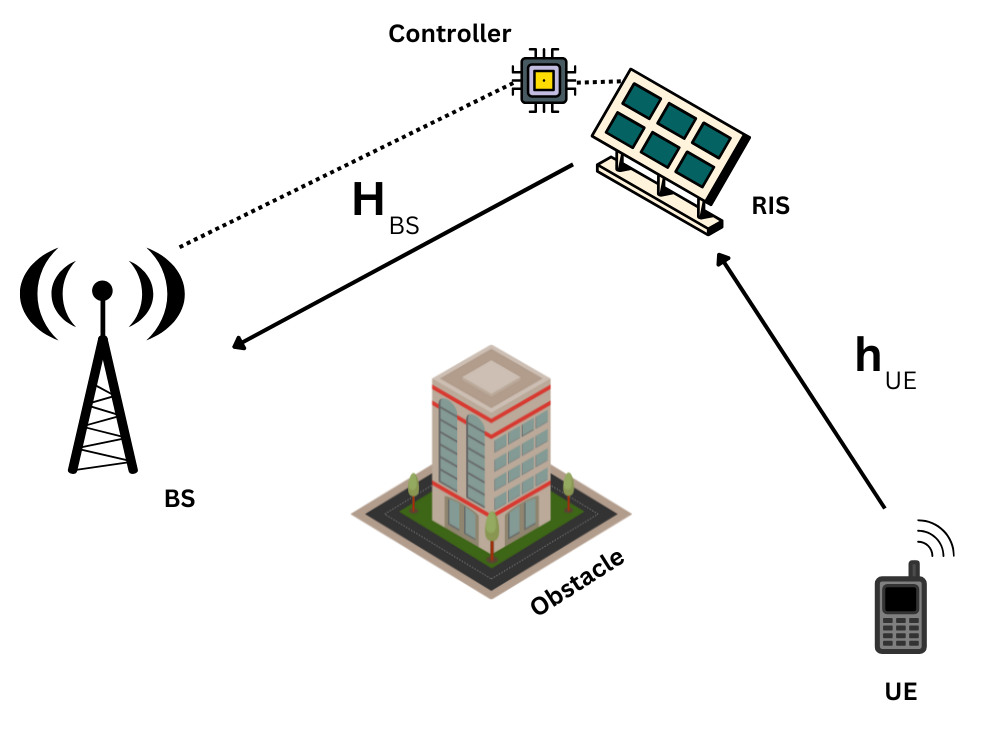
\includegraphics[width =\textwidth]{Figures/system_setup_no_angles_no_h_d.png}
            \end{column}
            \begin{column}{0.49\textwidth}
                \onslide <1-2> The received signal at the base station (BS) is: 
                \begin{equation*}
                    \mathbf y = \sqrt{P}\mathbf{H}_{\text{BS}} \boldsymbol{\Theta} \mathbf{h}_{\text{UE}} s + \bold{w}
                \end{equation*}
                where $P$ is the transmit power of the user, $||{s}||^2 = 1$, $\mathbf{w} \sim \mathcal{CN}(0,\sigma_w^2)$ and $\boldsymbol{\Theta} = $\text{diag}($\boldsymbol{\Phi}$), with $\boldsymbol{\Phi} =[e^{j\theta_0},....,e^{j\theta_{N_{RIS}-1}}]$, where the $\theta_{i}$ are the phase shifts introduced by the RIS, $ i \in [0,N_{RIS}-1]$.\\ 
                \onslide <2>
                \vspace{5mm}
                We write the full channel:
                \begin{equation*}
                    \mathbf h(\boldsymbol{\Phi}) = \bold{H}_{\text{BS}} \text{diag}(\boldsymbol{\Phi}) \mathbf{h}_{\text{UE}}
                \end{equation*}  
            \end{column}
        \end{columns}
    \end{frame}

    %------------------------------------------------

    \begin{frame}
        \frametitle{System Model}
        \framesubtitle{Codebook design}
        We use a DFT codebook, and we separate the codebook into two parts: 
        \begin{itemize}
            \item \onslide <2-4> $\boldsymbol{\Psi}_{1}^{\mathrm N_p} = [\boldsymbol{\Psi}_1,\ldots,\boldsymbol{\Psi}_{\mathrm N_p}]$, codebook for pilots, wide beams, where $|\boldsymbol{\Psi}_{1}^{\mathrm N_p}| = \mathrm N_p$.
            \item \onslide <3-4> $\boldsymbol{\Phi}_{1}^{\mathrm N_c} = [\boldsymbol{\Phi}_1,\ldots,\boldsymbol{\Phi}_{\mathrm N_c}]$, codebook for communication, narrows beams, where $|\boldsymbol{\Phi}_{1}^{\mathrm N_c}| = \mathrm N_c$.
        \end{itemize}
        \vspace{5mm}
        \onslide <4> What is the configuration of the RIS that maximises the rate?
    \end{frame}

    %------------------------------------------------

    \section{State-of-the-art}

    %------------------------------------------------    

    \begin{frame}
        \frametitle{State-of-the-art}
        \begin{definition}[Rate]
            \onslide <1-3> We want to get a higher coverage, which leads to maximizing the rate:
            \begin{equation*}
                \mathrm{R} 
                = 
                \max_{i \in \llbracket \mathrm N_c \rrbracket} 
                \left [
                    \log_2 \left ( 1+\frac{P \|\mathbf{H}_{\text{BS}} \text{diag}({\boldsymbol{\Phi}_{i}}) \mathbf{h}_{\text{UE}}\|_2^2 }{\sigma_{\mathrm w}^2} \right )
                \right ]
            \end{equation*}
            % where $\bold{h}$ the full channel.
        \end{definition}
        \begin{columns}
            \onslide <2-3> \begin{column}{0.45\textwidth}
                \begin{block}{CSI}
                    Channel estimation is challenging.
                \end{block}
            \end{column}
            \begin{column}{0.45\textwidth}
                \onslide <3> \begin{block}{No CSI}
                    "Blind" method.
                \end{block}
            \end{column}
        \end{columns}
    \end{frame}

    %------------------------------------------------

    \begin{frame}
        \frametitle{State-of-the-art}
        \framesubtitle{Blind Beamforming}
        Search for the optimal configuration (codeword $\boldsymbol{\Phi}_{\text{opt}} \in \boldsymbol{\Phi}_{1}^{\mathrm N_c}$) of RIS over the possible configurations (communication codebook $\boldsymbol{\Phi}_{1}^{\mathrm N_c}$) :
        \vspace{3mm}
        \begin{itemize}
            \item <1-> Exhaustive search over the codebook.
            \begin{itemize}
                \item Huge overhead 
            \end{itemize}
             \item <2-> Hierarchical : Need to create a specific codebook.
             \begin{itemize}
                \item Low overhead. 
                \item Might not reach the optimal configuration because of its shape (binary tree). 
            \end{itemize}
        \end{itemize}
    \end{frame}

    %------------------------------------------------

    \section{Bayesian Classifier}

    %------------------------------------------------

    \begin{frame}
        \frametitle{Bayesian Classifier}
        \framesubtitle{Protocol}
        \onslide <1-6> For a channel realization $\mathbf H$, we define $\boldsymbol\Phi(\mathbf H)$ as the class that assigns for this channel the best communication codeword $\boldsymbol\Phi \in \boldsymbol\Phi_{1}^{N_c}$:
        \begin{equation*}
            \boldsymbol{\Phi}(\mathbf H) = \{\boldsymbol{\Phi} \in \boldsymbol{\Phi}_{1}^{\mathrm N_c} : \boldsymbol{\Phi} = \argmax_{\boldsymbol{\Phi} \in \boldsymbol{\Phi}_{1}^{\mathrm N_c}} \!\ (||\bold{h}(\boldsymbol{\Phi})||_2^2)\}.
            % \boldsymbol{\Phi}(\mathbf H) = \{\boldsymbol{\Phi} \in \boldsymbol{\Phi}_{1}^{\mathrm N_c} : \boldsymbol{\Phi} = \argmax_{\boldsymbol{\Phi} \in \boldsymbol{\Phi}_{1}^{\mathrm N_c}} \bigl(\lVert\bold{h}(\boldsymbol{\Phi}) \rVert_2^2\bigr)\}.
        \end{equation*}
        \onslide <2-6> We introduce a probability vector associated with the communication codebook $\boldsymbol\Phi_{1}^{N_c}$:
        \begin{equation*}
            \mathbf{p}(\boldsymbol\Phi(\mathbf{H})) = \Big[\mathbf{p}(\boldsymbol\Phi(\mathbf{H}) = \boldsymbol\Phi_{1}), \ldots, \mathbf{p}(\boldsymbol\Phi(\mathbf{H}) = \boldsymbol\Phi_{N_c})\Big].
        \end{equation*}
        \onslide <3-6> The UE sends a pilot symbol $s_k$.
        \onslide <4-6> The RIS uses the index of a pilot codeword $\pi_k \in \llbracket 1,N_p \rrbracket$, i.e., $\boldsymbol\Psi_{\pi_k} \in \boldsymbol{\Psi}_{1}^{N_p}$ defined by the BS.
        \onslide <5-6> The BS computes the Received Signal Energy (RSE) where $k \in \llbracket 1,\mathrm N_p \rrbracket$:
        \begin{equation*}
            \mathrm Y_k = \mathbf y_k \mathbf y_k^{H}
        \end{equation*}
        \onslide <6> At each time step $t$, update the posteriori probability with knowledge over all received feedbacks: 
        \begin{equation*}
            \mathbf{p}(\boldsymbol{\Phi}(\mathbf H)| \mathrm Y_{1}^{\mathrm t},\boldsymbol{\Psi}_{1}^{\mathrm t})\triangleq [\mathbf{p}(\boldsymbol{\Phi}_1| \mathrm Y_{1}^{\mathrm t},\boldsymbol{\Psi}_{1}^{\mathrm t}), \cdots, \mathbf{p}(\boldsymbol{\Phi}_{\mathrm N_c}| \mathrm Y_{1}^{\mathrm t},\boldsymbol{\Psi}_{1}^{\mathrm t})]
        \end{equation*}
    \end{frame}

    %------------------------------------------------

    \begin{frame}
        \frametitle{Bayesian Classifier}
        \framesubtitle{Naive Bayes Classifier}        
        \begin{block}{Classification}
            Let $\mathrm L_{p}$ be the amount of the received samples, the Bayes optimal classifier is:
            \begin{equation*}
                % \arg\!\!\max_{c \in [1;N_c]} p(\boldsymbol{\Phi}(\mathbf H)| \mathbf Y_{1}^{\mathrm L_p},\boldsymbol{\Psi}_{1}^{\mathrm L_p})
                \argmax_{c \in \llbracket 1,\mathrm N_c \rrbracket} \!\ \mathbf{p}(\boldsymbol{\Phi}(\mathbf H)| \mathrm Y_{1}^{\mathrm L_p},\boldsymbol{\Psi}_{1}^{\mathrm L_p})
            \end{equation*}
        \end{block}
    \end{frame}

    %------------------------------------------------

    \begin{frame}
        \frametitle{Bayesian Classifier}
        \framesubtitle{Naive Bayes Classifier}  
        \begin{block}{Objective}
            \onslide<1-2>{
                Our main purpose is to find the optimal configuration $\Phi_{\text{opt}}$ while minimizing the number of required pilots $\boldsymbol\Psi \in \boldsymbol{\Psi}_{1}^{\mathrm N_p}$:
                \begin{equation*}
                    \mathrm L_{\text{min}} = \min \{\mathrm L_p : \| \mathbf{p}(\boldsymbol{\Phi}(\mathbf H) | \mathrm Y_1^{\mathrm L_p},\boldsymbol{\Psi}_1^{\mathrm L_p}) \|\infty = 1\}
                \end{equation*}
            }
            \onslide<2>{
                We introduce a fixed degree of precision $\delta\in [0;1]$ and we need to minimize $\mathrm L_{\text{p}}$ st. the probability of correct classification respects a certain precision:
                \begin{equation*}
                    \mathrm L_{\text{min}} = \min \{\mathrm L_p : \| \mathbf{p}(\boldsymbol{\Phi}(\mathbf H) | \mathrm Y_1^{\mathrm L_p},\boldsymbol{\Psi}_1^{\mathrm L_p}) \|\infty >1-\delta\}
                \end{equation*}
            }
        \end{block}
    \end{frame}
    %------------------------------------------------
    
    \section{Proposed approach: Reinforcement Learning}

    %------------------------------------------------

    \begin{frame}
        \frametitle{Proposed approach: Reinforcement Learning}
        \framesubtitle{State, Action, and Reward Flow}
        \begin{columns}
    
            % First Column (First Diagram)
            \column{0.6\textwidth}
            \only<1->{ % First diagram appears first
            \scalebox{0.75}{ % Scale down the diagram to fit the slide
            \begin{tikzpicture}[
                node distance=1.5cm and 2.5cm, 
                every node/.style={draw, minimum width=2.8cm, minimum height=1cm, align=center, font=\scriptsize}, 
                every path/.style={thick, ->, >=stealth}
            ]
        
                % Define Nodes
                \node (init) [rectangle, rounded corners, fill=blue!15] {Initial State\\ $S_{\text{init}} = \mathbf{p}(\boldsymbol{\Phi}(\mathbf{H})) = [\frac{1}{N_c},\cdots,\frac{1}{N_c}]$};
                
                \node (action) [rectangle, rounded corners, below=1cm of init, fill=green!20] {Choose Pilot Codeword $\boldsymbol{\Psi} \in \boldsymbol{\Psi}_{1}^{\mathrm N_p}$};
        
                \node (state_new) [rectangle, rounded corners, below=1cm of action, fill=blue!15] {New State};
        
                \node (reward) [rectangle, rounded corners, below=1cm of state_new, fill=red!20] {Reward: -1 if not Terminal State};
        
                \node (terminal) [rectangle, rounded corners, right=4.5cm of state_new, fill=red!20] {Terminal State \\ (Correct Codeword Found) \\ Reward = 0};
        
                % Draw Arrows
                \draw[arrow] (init.south) -| (action.north);  
                \draw[arrow] (action.south) -- (state_new.north);  
                \draw[arrow] (state_new.south) -- (reward.north);  
        
                % Loop back to action if not terminal
                \draw[arrow] (reward.west) -| (-2.5,-2.04) -- (action.west); 
        
                % Transition to terminal state if condition met
                \draw[arrow] (state_new.east)  -- node[midway, above =.2, rounded corners] {If \\ $\| \mathbf{p}(\boldsymbol{\Phi}(\mathbf H) | \mathrm Y_1^t,\boldsymbol{\Psi}_1^t) \|\infty >1-\delta$} 
                    (terminal.west);
        
            \end{tikzpicture}
            }
            }
            
            % Second Column (Second Diagram)
            \column{0.3\textwidth}
            \only<2->{ % Second diagram appears on next step
            \scalebox{0.65}{ % Scale down the diagram
            \begin{tikzpicture}[
                node distance=2cm and 3cm,
                every node/.style={font=\small},
                block/.style={rectangle, draw, minimum width=2.5cm, minimum height=1.2cm, align=center},
                arrow/.style={draw, thick, ->, >=stealth}
            ]
            
            % Nodes
            \node [fill=yellow!30] (agent) at (0,2) [block] {Agent};
            \node [fill=yellow!30] (env) at (0,-2) [block] {Environment};
            \node (state_t) at (3,0.5) {State $S_t$};
            \node (reward_t) at (3,-0.5) {Reward $R_t$};
            \node (state_t1) at (-3,0.5) {State $S_{t+1}$};
            \node (reward_t1) at (-3,-0.5) {Reward $R_{t+1}$};
            
            % Arrows
            \draw[arrow] (state_t) |- (agent);
            \draw[arrow] (agent) -| (state_t1);
            \draw[arrow] (reward_t1) |- (env);
            \draw[arrow] (env) -| (reward_t);
            
            \end{tikzpicture}
            }
            }
        \end{columns}
    \end{frame}

    %------------------------------------------------
    
    \begin{frame}
        \frametitle{Proposed approach: Reinforcement Learning}
        \framesubtitle{Stochastic shortest path problem}
        \begin{block}{Policy}
            A policy $\pi(S)$ determines which action $A$ is chosen in a given state $S$:
            \begin{equation*}
                \pi(S) = A
            \end{equation*}
        \end{block}
        \pause
        \begin{block}{Objective}
            The goal is to reach a terminal state where the probability of correct classification respects a fixed degree of precision $\delta \in [0;1]$:
            \begin{equation*}
                \mathrm L_{\text{min}} = -\sum_{t=0}^{\infty} R_t
            \end{equation*}
        \end{block}
    \end{frame}

    %------------------------------------------------

    \begin{frame}
        \frametitle{Proposed approach: Reinforcement Learning}
        \framesubtitle{Q-Learning: Value Function and Policy}
        \begin{block}{Q-function} 
            The Q-value function represents the expected cumulative reward when taking action $A_t$ in state $S_t$:
            \begin{equation*}
                Q(S_t, A_t) = \mathbb{E}_{\mathbf H,\mathbf w}\left[\sum_{k=0}^{\infty} R_{t+k+1} \mid S_t = S, A_t = A\right]
            \end{equation*}
        \end{block} 
        \pause
        \begin{block}{Bellman Equation}
            The Q-values are updated using the Bellman equation:
            \begin{equation*}
                Q(S_t, A_t) \leftarrow {(1-\alpha) Q(S_t, A_t) + \alpha[{R}_{t+1} + \max_{A}Q(S_{t+1}, A)]}
            \end{equation*}
            where $\alpha \in [0,1]$ is the learning rate.
        \end{block}
    \end{frame}

    %------------------------------------------------

    \begin{frame}
        \frametitle{Proposed approach: Reinforcement Learning}
        \framesubtitle{Q-Learning: Optimal policy}
        \begin{block}{Optimal Policy}
            The optimal policy is obtained by selecting the action that maximizes the expected reward :
            \begin{equation*}
                \pi^*(S) = \arg\max_{A} Q^*(S,A)
            \end{equation*}
        \end{block}
        \pause
        \begin{block}{Objective}
            Thus, our goal is to find the optimal policy $\pi^*$ that maximizes the cumulative reward despite randomness in the channel and noise. We rewrite our objective:
            \begin{equation*}
                \mathrm L^{*} = \max_{\pi}
                 \mathbb{E}_{\bold{H},\bold{w}}
                \left[
                    \sum_{t=0}^{\infty} R_t 
                \right]
            \label{eq:L_min_*}
            \end{equation*}
        \end{block}
    \end{frame}

    %------------------------------------------------

    \begin{frame}
        \frametitle{Proposed approach: Reinforcement Learning}
        \framesubtitle{From Q-Learning to Deep Q-Learning}
        \begin{itemize}[<+->]
            \item The state space was discretized \cite{chene-};
            \item Transitions were determined using Euclidean distances to predefined states;
            \item This approach became unreliable in high dimensions;
            \item Small variations led to misclassifications among similar codewords.
        \end{itemize}
        \vfill
        \vspace{9mm}
        {\tiny{[1]: T. Chêne, O. Bounhar, G. R.-B. Othman, and O. Damen, “Adaptive Passive
        Beamforming in RIS-Aided Communications with Q-Learning,” in 2025 IEEE Wireless
        Communications and Networking Conference (WCNC).
        Milan, Italy : IEEE, 2025, pp.
        1–6.}}  
    \end{frame}

    %------------------------------------------------

    \begin{frame}
        \frametitle{Proposed approach: Reinforcement Learning}
        \framesubtitle{Deep Q-Neural Netwok}
        \begin{itemize}[<+->]
            \item Replacing the Q-table with a neural network (NN) that generalizes over continuous state spaces.
        \end{itemize}
        \begin{figure}
            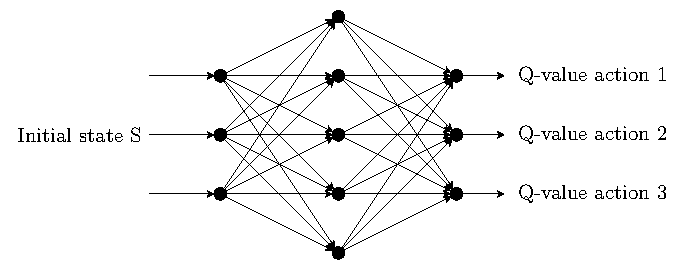
\includegraphics[width = 0.65\textwidth]{Tikz/dqn.pdf}
        \end{figure}
    \end{frame}

    %------------------------------------------------

    \begin{frame}
        \frametitle{Proposed approach: Reinforcement Learning}
        \framesubtitle{Deep Q-Neural Netwok}
        Deep Q-Learning (DQL) uses two NN:
        \begin{itemize}[<+->]
            \item Evaluation network (Eval-Net) parameterized by the NN weights $\theta^{(eval)}$,
            \item Target network (Target-Net) parameterized by NN weights $\theta^{(target)}$.
        \end{itemize}
        \pause
        \begin{block}{Approximation of the Q-function}
            The Q-function approximation can thus be expressed as:
            \begin{equation}
                Q_{\text{eval}}(S, A; \theta^{(eval)}) \approx \mathbb{E}\left[R + \gamma \max_{A'} Q_{\text{target}}(S', A'; \theta^{(target)})\right],
            \end{equation}
        \end{block}
    \end{frame}

    %------------------------------------------------

    \begin{frame}
        \frametitle{Proposed approach: Reinforcement Learning}
        \framesubtitle{Deep Q-Learning Algorithm}
        \begin{figure}
            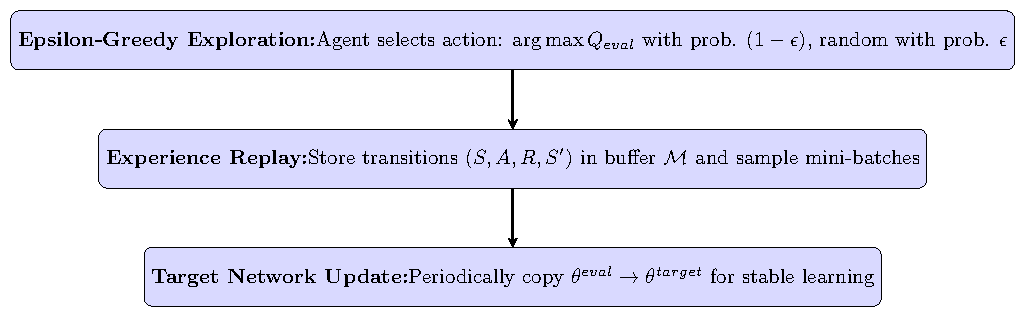
\includegraphics[width = 0.9\textwidth]{Tikz/trainingDQN.pdf}
        \end{figure}
    \end{frame}
        
    %------------------------------------------------

    \begin{frame}
        \frametitle{Proposed approach: Reinforcement Learning}
        \framesubtitle{Deep Q-Neural Netwok}
        \begin{block}{Network Optimization}
            The Q-network is trained by minimizing the mean squared error (MSE) loss, defined as:
            \begin{equation}
            \mathcal{L}(\theta) = \mathbb{E} \big[ \smash{(Q_{\text{target}} - Q_{\text{eval}}(S, A; \theta^{(\text{eval})}))^2} \big],
            \label{eq: loss}
            \end{equation}
            with:
            \begin{equation}
                Q_{\text{target}} = R + \gamma \max_{\Psi} Q_{\text{target}}(S', \Psi; \theta^{(target)}).
            \end{equation}
        \end{block}
    \end{frame}
    
    %------------------------------------------------

    \section{Simulation results}

    %------------------------------------------------

    % \begin{frame}
    %     \frametitle{Simulation results}
    %     \framesubtitle{Comparison to other benchmarks}
    %     % \begin{figure}
    %         \centering
    %         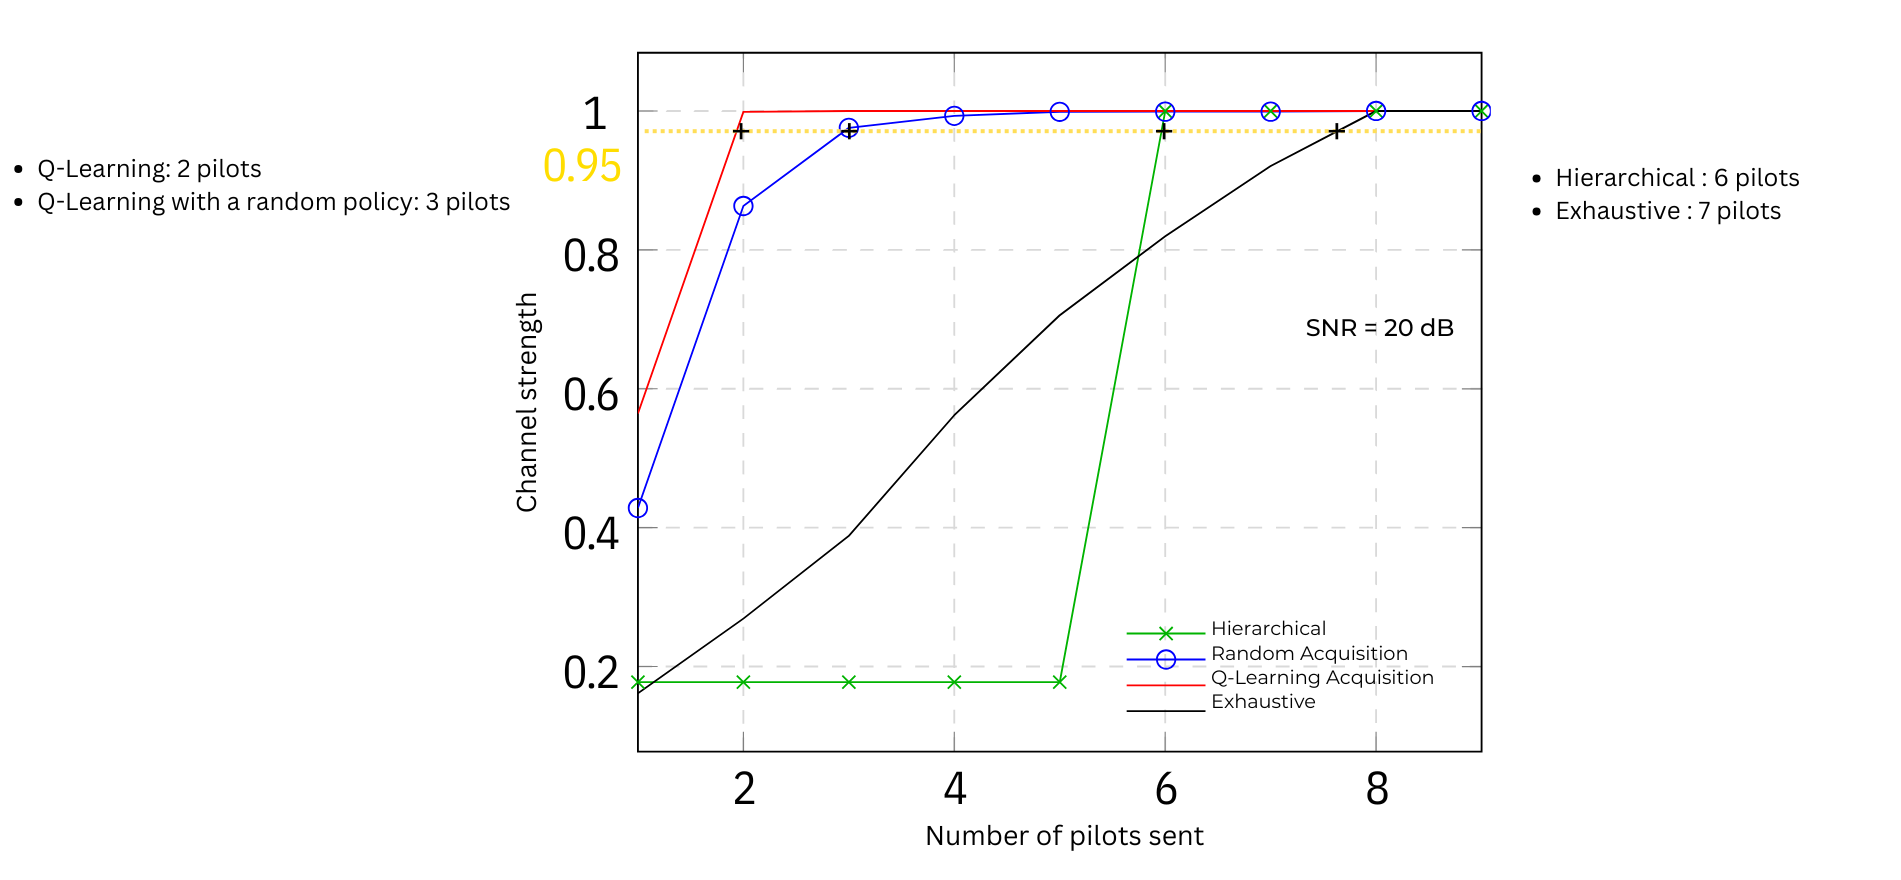
\includegraphics[width = 0.9\textwidth]{Figures/Soutenance MICAS - Oumaïma Bounhar.png}
    %         % \caption{\centering \parbox{0.6\textwidth}{Comparison of benchmarks for selecting the optimal configuration for the RIS.}}
    %     % \end{figure}
    % \end{frame}

    %------------------------------------------------
    
    \begin{frame}
        \frametitle{Simulation results}
        \framesubtitle{Comparison to other benchmarks}
        % \begin{figure}
            \centering
            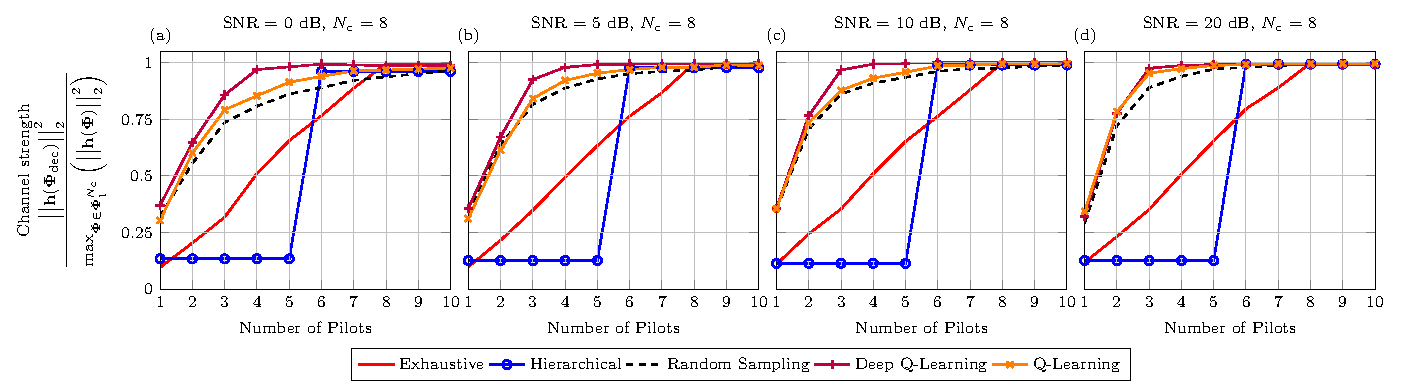
\includegraphics[width = \textwidth]{Figures/8_codewords_plot.pdf}
            % \caption{\centering \parbox{0.6\textwidth}{Comparison of benchmarks for selecting the optimal configuration for the RIS.}}
        % \end{figure}
        \pause
        % \justifying
        \raggedright
        These results demonstrate that our proposed approach using Deep Q-Learning successfully minimizes pilot overhead, requiring at most $L^* = 4$ pilots in low-SNR conditions and only $L^* = 3$ pilots at moderate-to-high SNRs \cite{DQN}.

        {\tiny{[2]: O. Bounhar, T. Chene, G. R.-B. Othman, and O. Damen, “Deep q-learning for passive beamforming in ris-assisted mimo systems,” 2026.}}
    \end{frame}    

    %------------------------------------------------
    
    \begin{frame}
        \frametitle{Simulation results}
        \framesubtitle{Comparison to other benchmarks}
        % \begin{figure}
            \centering
            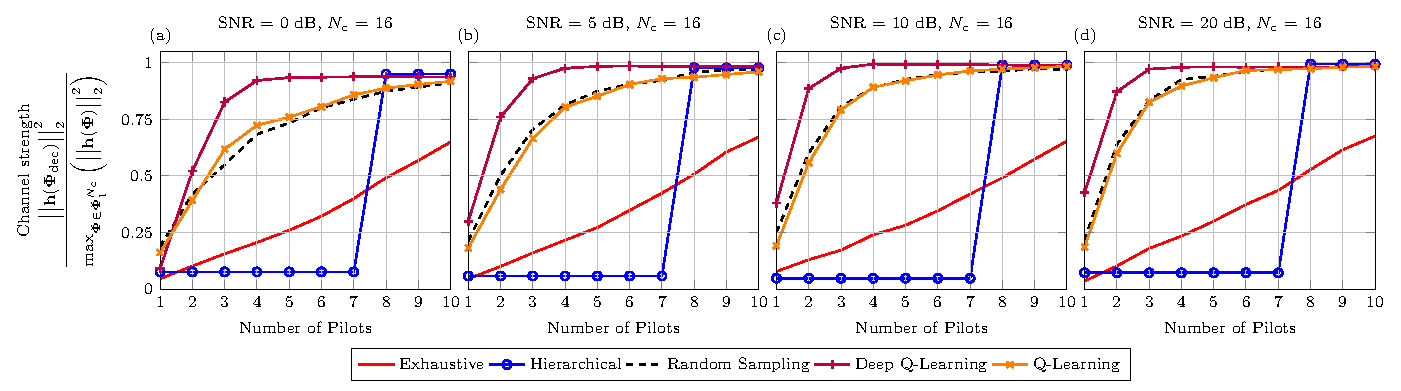
\includegraphics[width = \textwidth]{Figures/16_codewords_plot.pdf}
            % \caption{\centering \parbox{0.6\textwidth}{Comparison of benchmarks for selecting the optimal configuration for the RIS.}}
        % \end{figure}
        \pause
        % \justifying
        \raggedright
        These results were extended to a larger codebook size of $N_c = 16$, where our proposed approach continues to outperform benchmarks, requiring at most $L^* = 5$ pilots in low-SNR conditions and only $L^* = 4$ pilots at moderate-to-high SNRs \cite{DQN}.

        {\tiny{[2]: O. Bounhar, T. Chene, G. R.-B. Othman, and O. Damen, “Deep q-learning for passive beamforming in ris-assisted mimo systems,” 2026.}}
    \end{frame}    

    %------------------------------------------------

    \section{Sionna - Realistic channel generation and validation}

    %------------------------------------------------
    
    \begin{frame}
        \frametitle{Sionna - Realistic channel generation and validation}
        \framesubtitle{Comparison to Rayleigh fading}
        % \begin{figure}
            \centering
            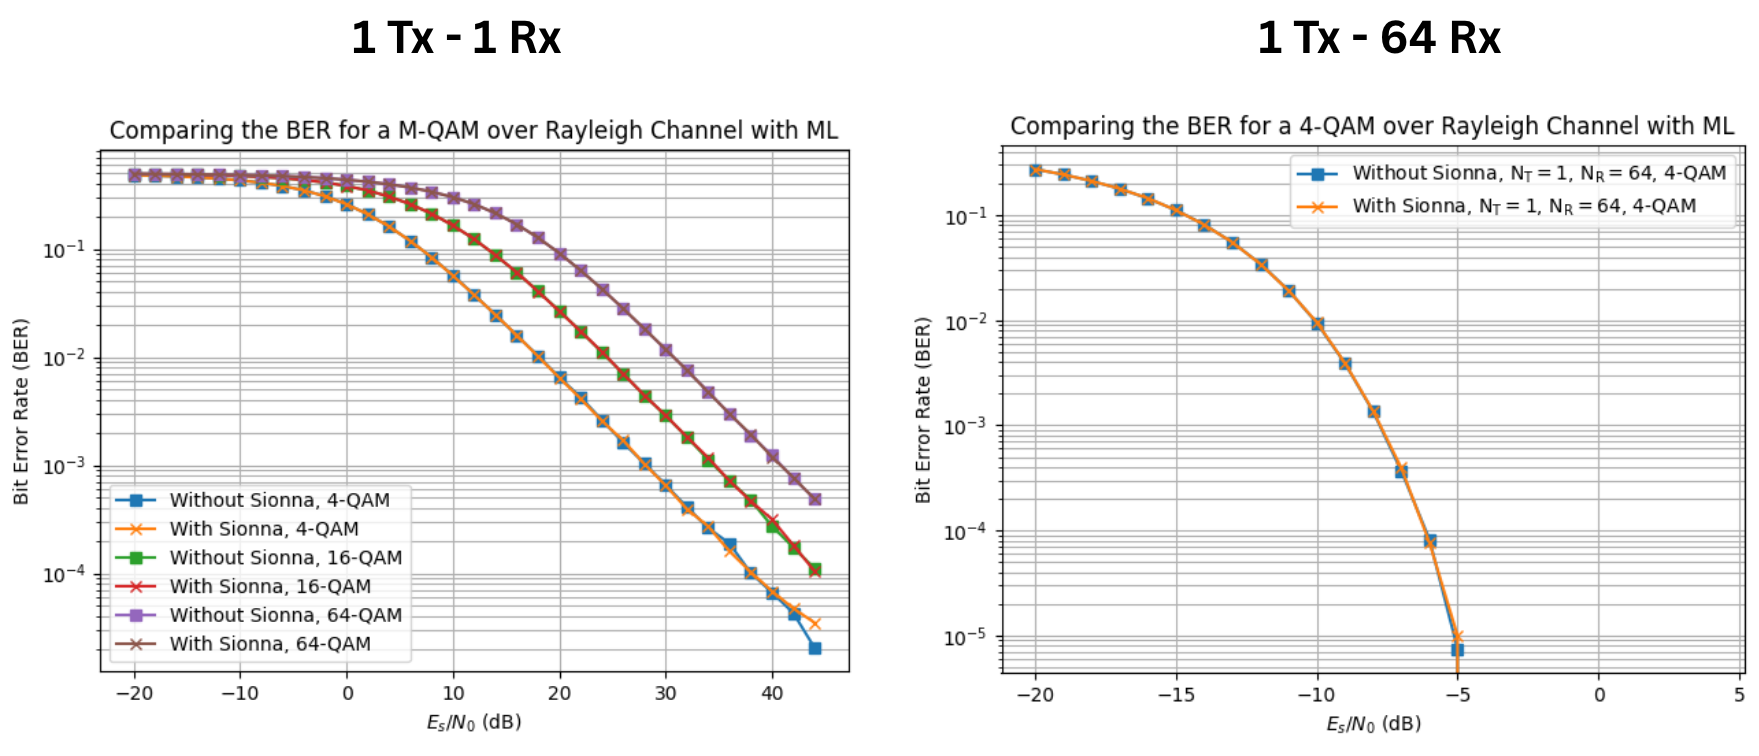
\includegraphics[width = 0.95\textwidth]{Figures/sionna_validated_simple_case.png}
            % \caption{\centering \parbox{0.6\textwidth}{Comparison of benchmarks for selecting the optimal configuration for the RIS.}}
        % \end{figure}
        
    \end{frame}    

    %------------------------------------------------
    
    \begin{frame}
        \frametitle{Sionna - Realistic channel generation and validation}
        \framesubtitle{Primer on electromagnetics: RIS reradiated field}
        \begin{columns}[T]
            % Left column
            \begin{column}{0.35\textwidth}
                \centering
                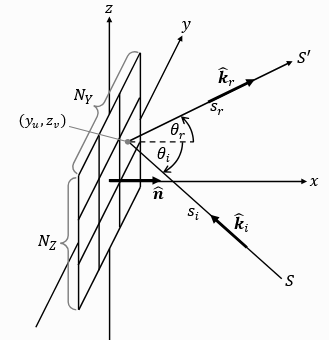
\includegraphics[width=0.95\textwidth]{Figures/RIS_fig_sionna.png}

                \vspace{0.1cm}
                {\scriptsize Incident and reradiated field from a RIS}
            \end{column}

                    % Right column
            \begin{column}{0.63\textwidth}

                \setlength{\abovedisplayskip}{2pt}
                \setlength{\belowdisplayskip}{2pt}
                \setlength{\abovedisplayshortskip}{2pt}
                \setlength{\belowdisplayshortskip}{2pt}

                \vspace{-0.3cm}

                \small The reradiated field from the RIS at point $S'$ is given by:
                \begin{equation*}
                \small
                \mathbf{E}_{r}(S')
                =
                \sum_{u=1}^{N_y}
                \sum_{v=1}^{N_z}
                \Gamma_{u,v}\,
                G_{u,v}\,
                A_{u,v}\,
                \mathbf{p}_{u,v}
                \end{equation*}

                \vspace{-0.1cm}
                where:
                \begin{align*}
                \small
                G_{u,v}
                &=
                \frac{3\lambda}{16\pi}
                \left(1+\cos\theta_i^{u,v}\right)
                \left(1+\cos\theta_r^{u,v}\right),
                \\[0.35em]
                A_{u,v}
                &=
                \frac{
                e^{-j k_0 \left(s_i^{u,v}+s_r^{u,v}\right)}
                }{
                s_i^{u,v}s_r^{u,v}
                },
                \\[0.35em]
                \mathbf{p}_{u,v}
                &=
                E_{i,\theta}(S)\,
                \hat{\boldsymbol{\theta}}\!\left(\hat{\mathbf{k}}_r^{u,v}\right)
                +
                E_{i,\varphi}(S)\,
                \hat{\boldsymbol{\varphi}}\!\left(\hat{\mathbf{k}}_r^{u,v}\right)
                \end{align*}
                \vspace{-0.3cm}
                \begin{columns}[T,onlytextwidth]
                    \begin{column}{0.48\textwidth}
                        \begin{equation*}
                        s_i^{u,v}
                        =
                        \left\|
                        \mathbf{r}_{\mathrm{RIS}}^{u,v}
                        -
                        \mathbf{r}_{\mathrm{Tx}}
                        \right\|_2
                        \end{equation*}

                        \centering
                        {\small Tx--RIS distance}
                    \end{column}

                    \begin{column}{0.48\textwidth}
                        \begin{equation*}
                        s_r^{u,v}
                        =
                        \left\|
                        \mathbf{r}_{\mathrm{Rx}}
                        -
                        \mathbf{r}_{\mathrm{RIS}}^{u,v}
                        \right\|_2
                        \end{equation*}

                        \centering
                        {\small RIS--Rx distance}
                    \end{column}

                \end{columns}
            \end{column}
        \end{columns}
    \end{frame}

    %------------------------------------------------

    \begin{frame}
        \frametitle{Sionna - Realistic channel generation and validation}
        \framesubtitle{Why geometry strongly affects the RIS channel}

        \begin{center}
            \Large
            \[
            \boxed{
            \text{Path loss}
            \propto
            \frac{1}{s_i^{u,v}s_r^{u,v}}
            }
            \]
        \end{center}

        \vspace{0.5cm}

        \begin{alertblock}{Main message}
            For RIS-assisted propagation, the attenuation is controlled by the both segments Tx--RIS and RIS--Rx, and it is proportional to the product of these two distances:
            \[
            d_{\mathrm{Tx}\rightarrow\mathrm{RIS}}
            \times
            d_{\mathrm{RIS}\rightarrow\mathrm{Rx}}.
            \]
        \end{alertblock}

    \end{frame}
    %------------------------------------------------
    
    \begin{frame}
        \frametitle{Sionna - Realistic channel generation and validation}
        \framesubtitle{Configuring scene geometry and RIS activation}
        % \begin{figure}
            \centering
            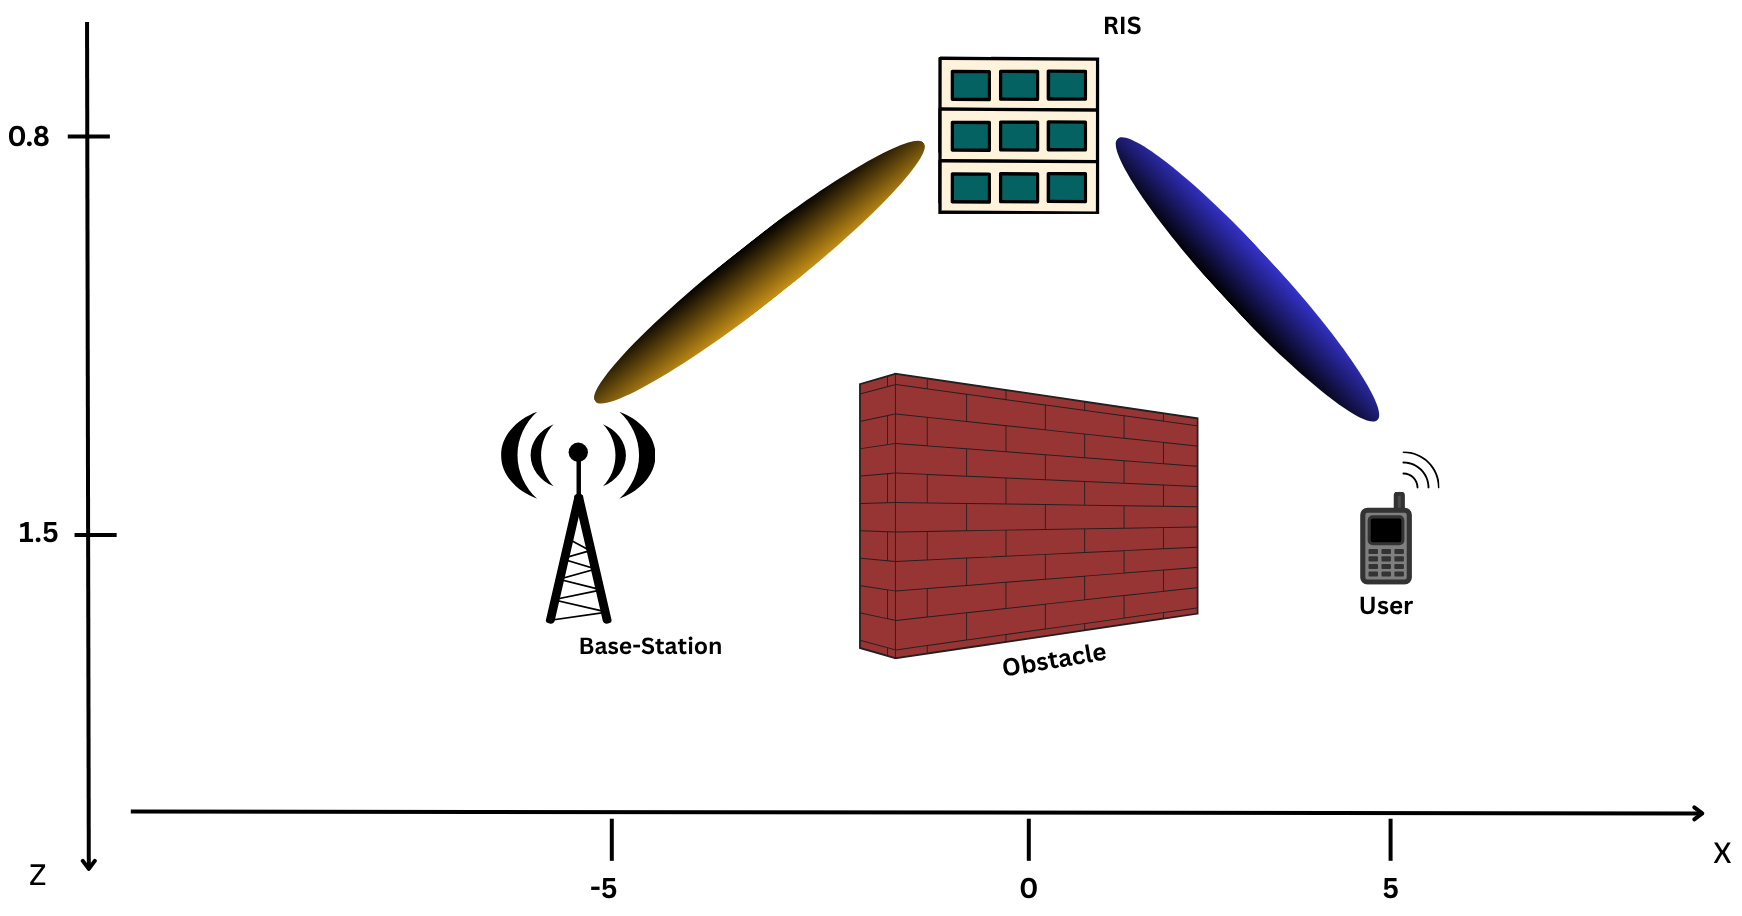
\includegraphics[width = 0.8\textwidth]{Figures/RIS_geomtery_0.png}
            % \caption{\centering \parbox{0.6\textwidth}{Comparison of benchmarks for selecting the optimal configuration for the RIS.}}
        % \end{figure}
        
    \end{frame}    

    %------------------------------------------------
    
    \begin{frame}
        \frametitle{Sionna - Realistic channel generation and validation}
        \framesubtitle{Configuring scene geometry and RIS activation}
        % \begin{figure}
            \centering
            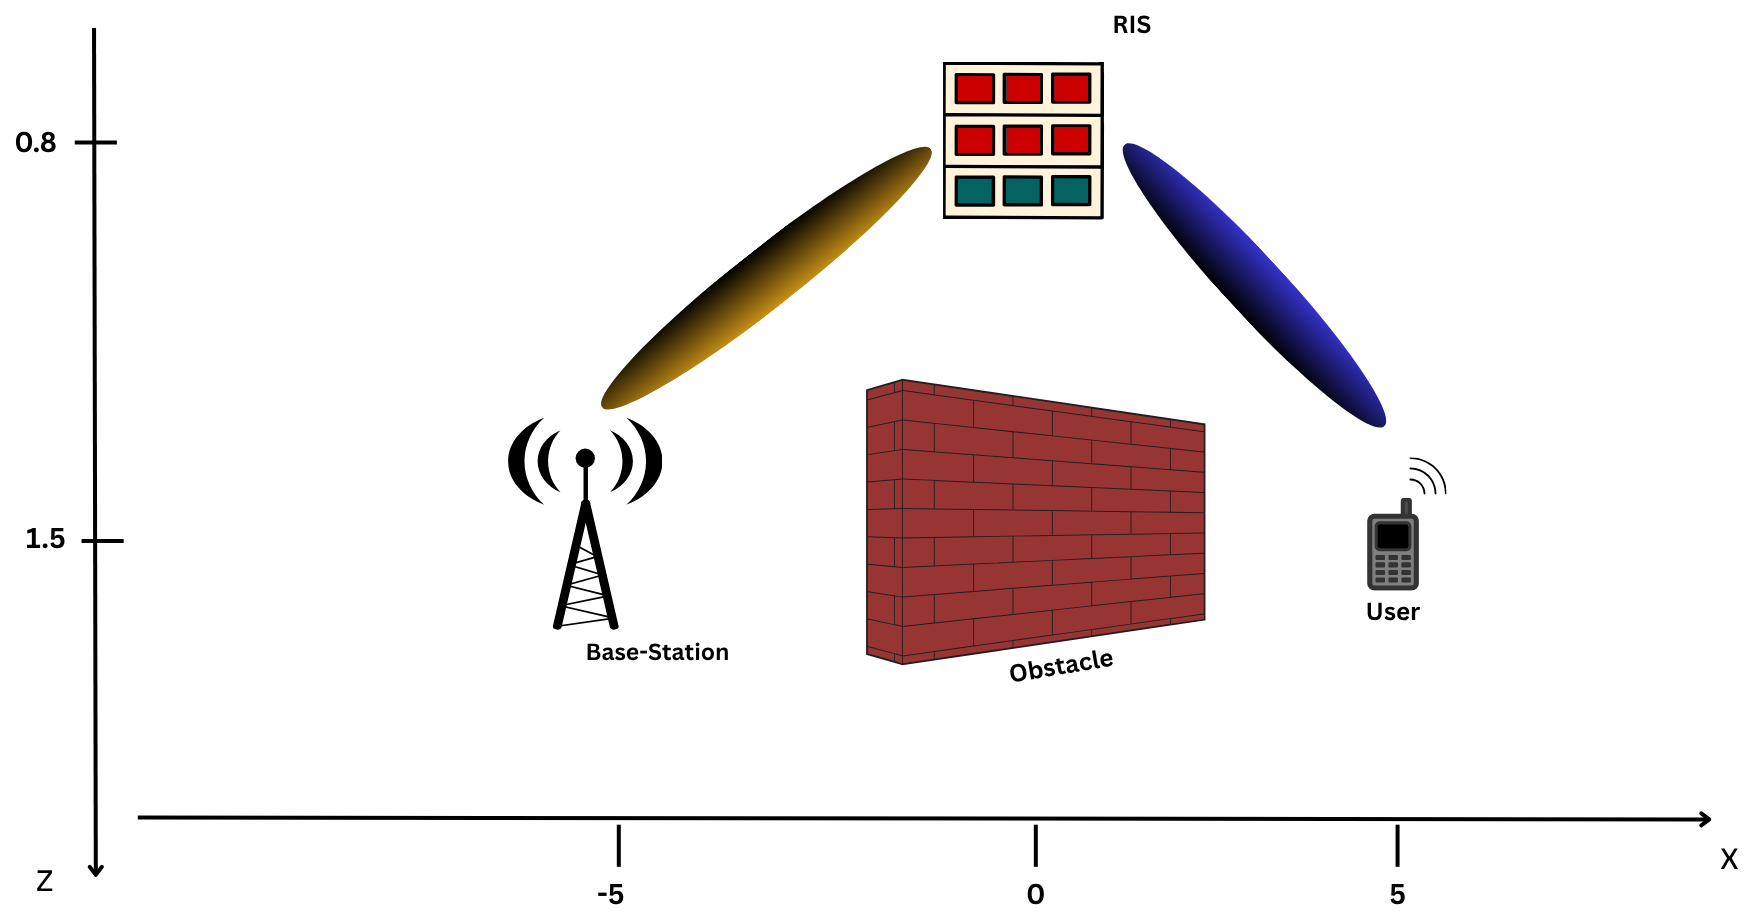
\includegraphics[width = 0.8\textwidth]{Figures/RIS_geomtery_1.png}
            % \caption{\centering \parbox{0.6\textwidth}{Comparison of benchmarks for selecting the optimal configuration for the RIS.}}
        % \end{figure}
        
    \end{frame}    

    %------------------------------------------------
    
    \begin{frame}
        \frametitle{Sionna - Realistic channel generation and validation}
        \framesubtitle{Configuring scene geometry and RIS activation}
        % \begin{figure}
            \centering
            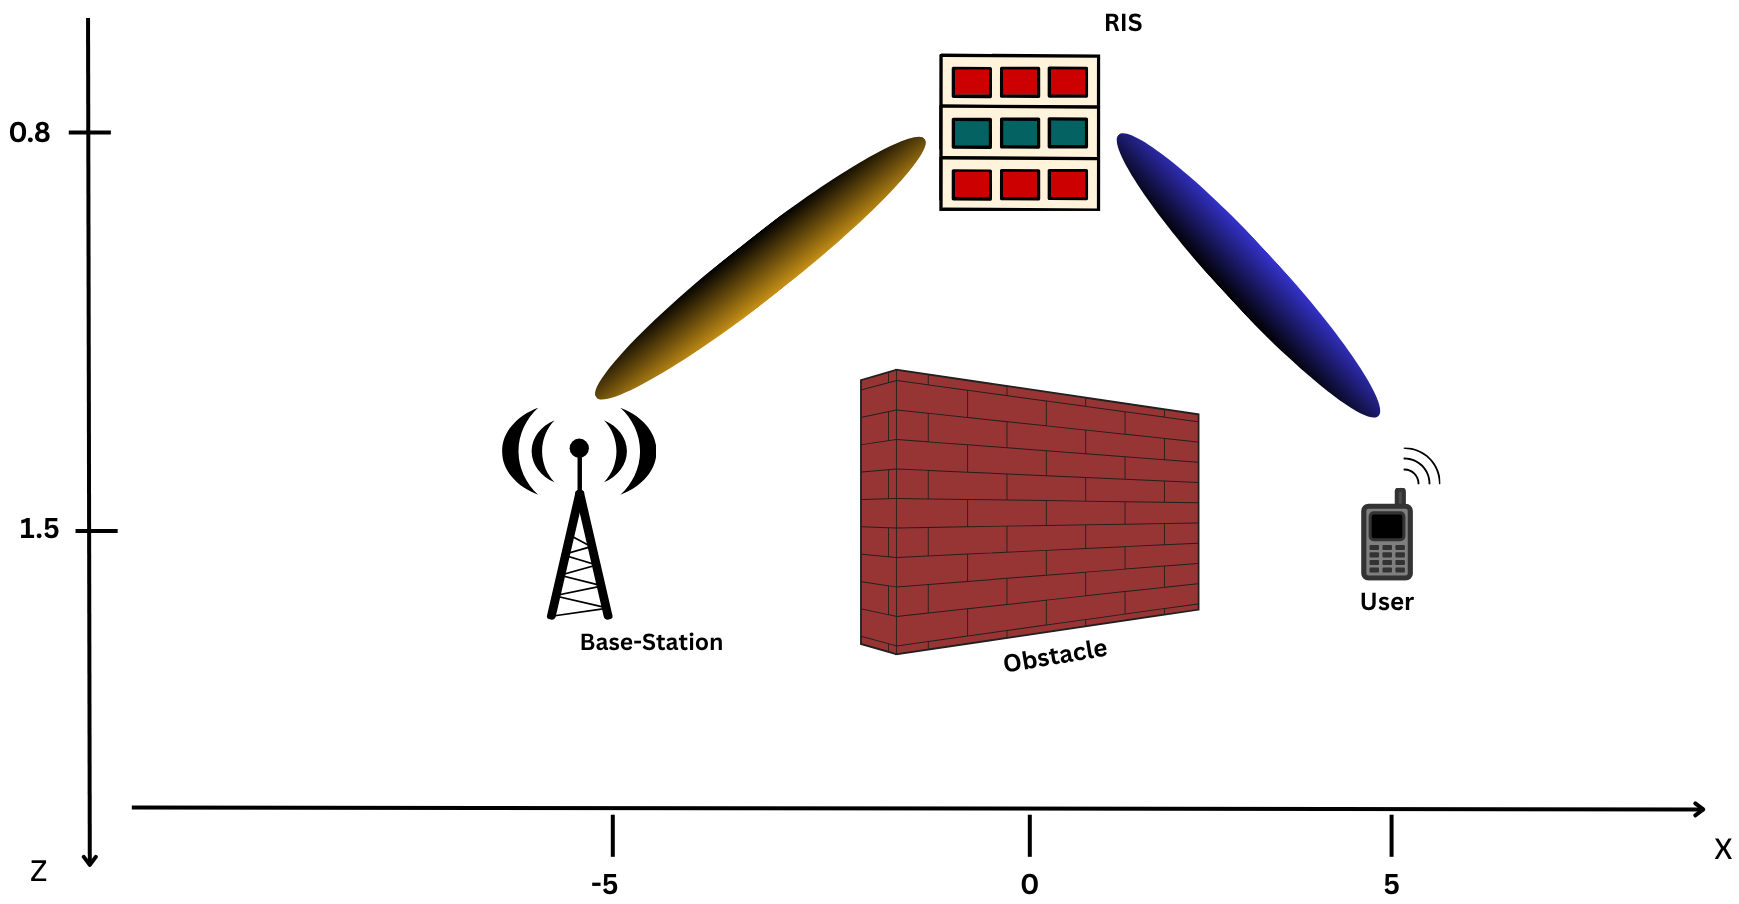
\includegraphics[width = 0.8\textwidth]{Figures/RIS_geomtery_2.png}
            % \caption{\centering \parbox{0.6\textwidth}{Comparison of benchmarks for selecting the optimal configuration for the RIS.}}
        % \end{figure}
        
    \end{frame}    

    %------------------------------------------------
    
    \begin{frame}
        \frametitle{Sionna - Realistic channel generation and validation}
        \framesubtitle{Configuring scene geometry and RIS activation}
        % \begin{figure}
            \centering
            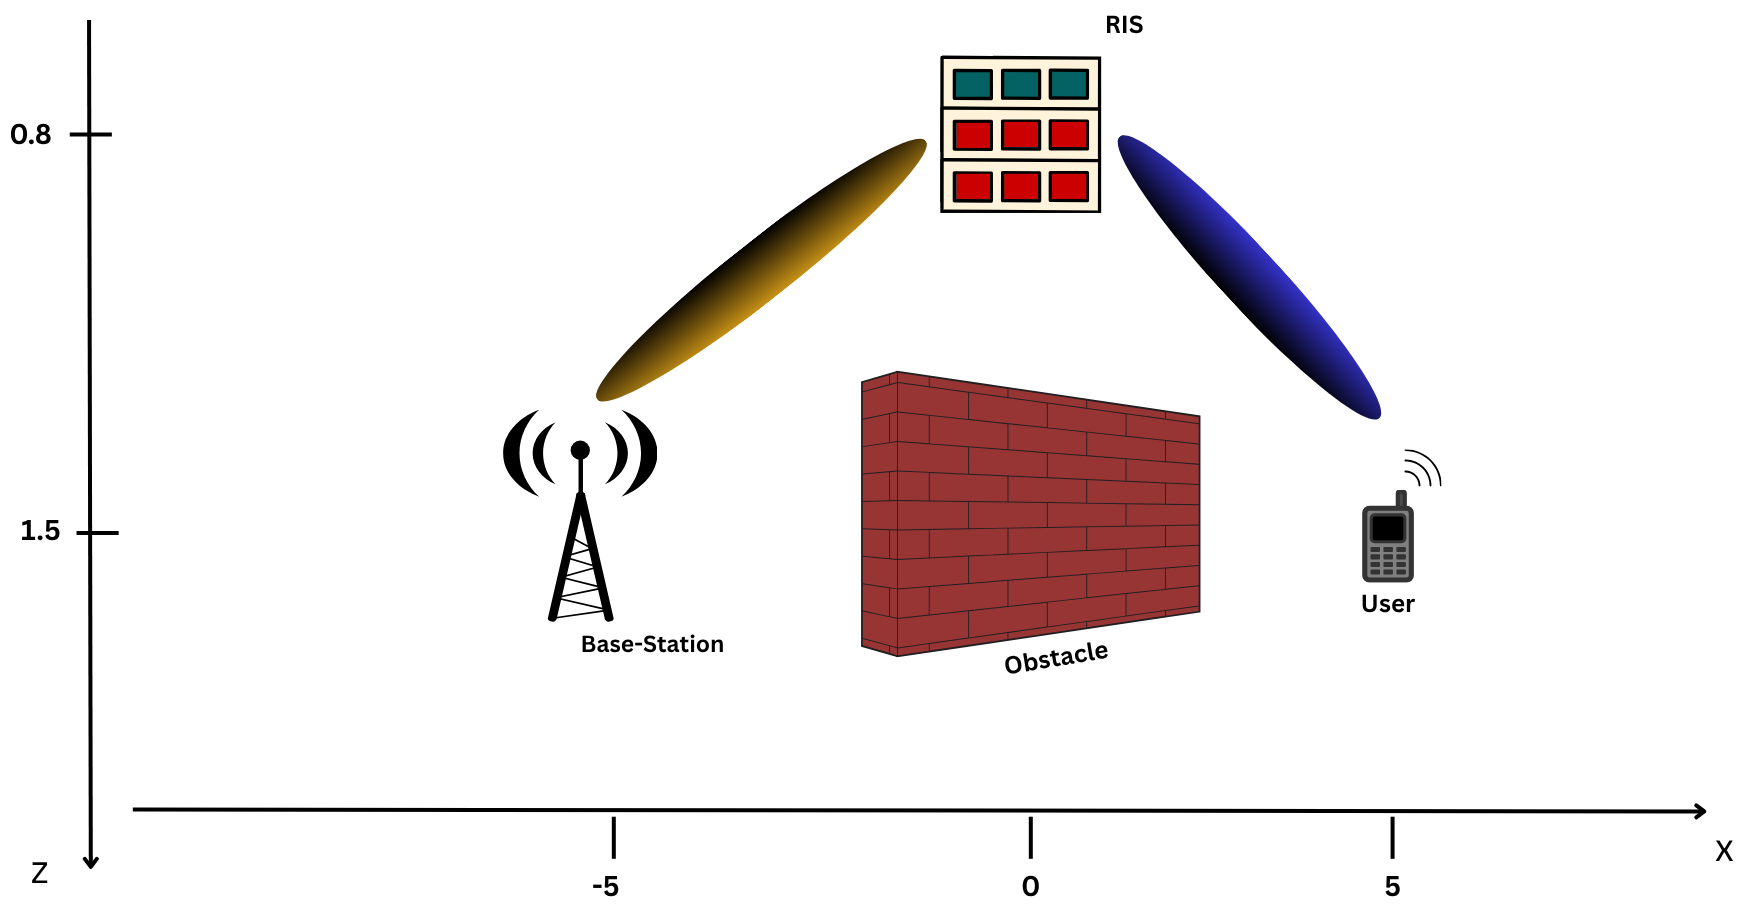
\includegraphics[width = 0.8\textwidth]{Figures/RIS_geomtery_3.png}
            % \caption{\centering \parbox{0.6\textwidth}{Comparison of benchmarks for selecting the optimal configuration for the RIS.}}
        % \end{figure}
        
    \end{frame}    

    %------------------------------------------------
    
    \begin{frame}
        \frametitle{Sionna - Realistic channel generation and validation}
        \framesubtitle{Channel computation workflow}
        % \begin{figure}
            \centering
            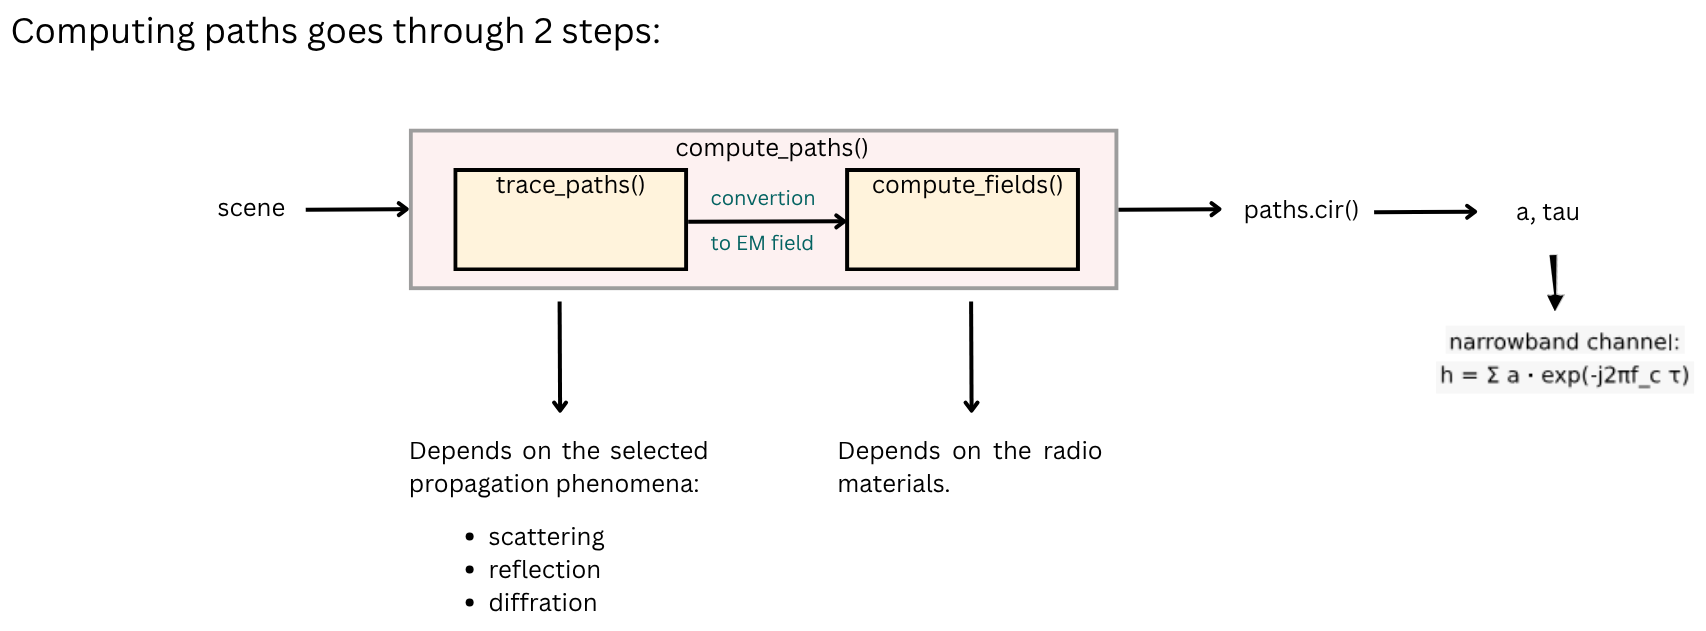
\includegraphics[width = 0.9\textwidth]{Figures/Channel_Compuation_Flow.png}
            % \caption{\centering \parbox{0.6\textwidth}{Comparison of benchmarks for selecting the optimal configuration for the RIS.}}
        % \end{figure}
        
    \end{frame}    

    %------------------------------------------------
    

    \begin{frame}
        \frametitle{Sionna - Realistic channel generation and validation}
        \framesubtitle{Toy example : 1D-DFT Codebook (3 codewords)}

        \begin{block}{DFT codebook construction}
            For $K$ codewords, the $k$-th 1D-DFT codeword is:
            \begin{equation*}
                \boldsymbol{\Phi}_k
                =
                \begin{bmatrix}
                1 &
                e^{j\theta_k} &
                e^{j2\theta_k} &
                \cdots &
                e^{j(N-1)\theta_k}
                \end{bmatrix}^{T},
                \qquad
                \theta_k
                =
                \frac{2\pi \text{k}}{\text{K}}.
            \end{equation*}
        \end{block}

        \vspace{0.2cm}

        \begin{alertblock}{Toy example}
            We use a 1D-DFT codebook with $K=3$ codewords:
            \begin{equation*}
                \boldsymbol{\Phi}^1_3
                =
                \left[
                \boldsymbol{\Phi}_1,
                \boldsymbol{\Phi}_2,
                \boldsymbol{\Phi}_3
                \right]
                =
                \begin{bmatrix}
                0 & 0 & 0 \\
                0 & -\frac{2\pi}{3} & \frac{2\pi}{3} \\
                0 & \frac{2\pi}{3} & -\frac{2\pi}{3}
                \end{bmatrix}.
            \end{equation*}
        \end{alertblock}

    \end{frame} 

    %------------------------------------------------
    
    \begin{frame}
        \frametitle{Sionna - Realistic channel generation and validation}
        \framesubtitle{Toy example : 1D-DFT Codebook (3 codewords)}
        % \begin{figure}
            \centering
            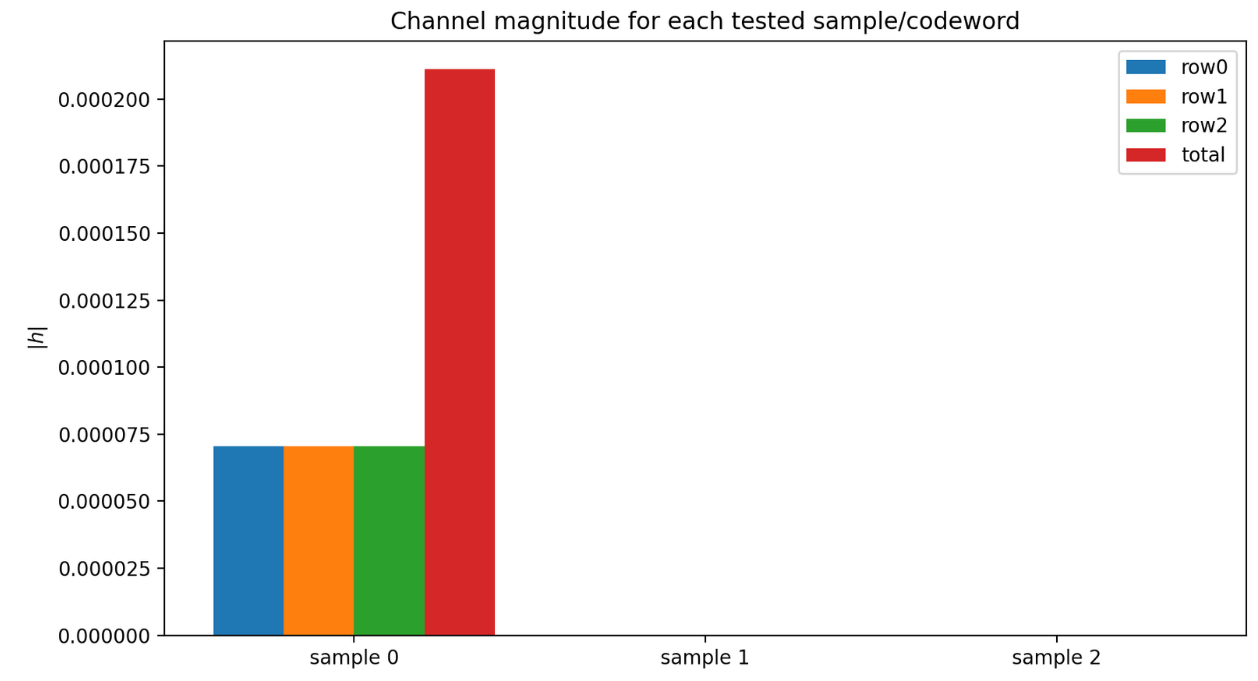
\includegraphics[width = 0.7\textwidth]{Figures/Channel_magnitude_simple_test.png}
            % \caption{\centering \parbox{0.6\textwidth}{Comparison of benchmarks for selecting the optimal configuration for the RIS.}}
        % \end{figure}
    \end{frame}

    %------------------------------------------------
    
    \begin{frame}
        \frametitle{Sionna - Realistic channel generation and validation}
        \framesubtitle{Generated channel}
        % \begin{figure}
            \centering
            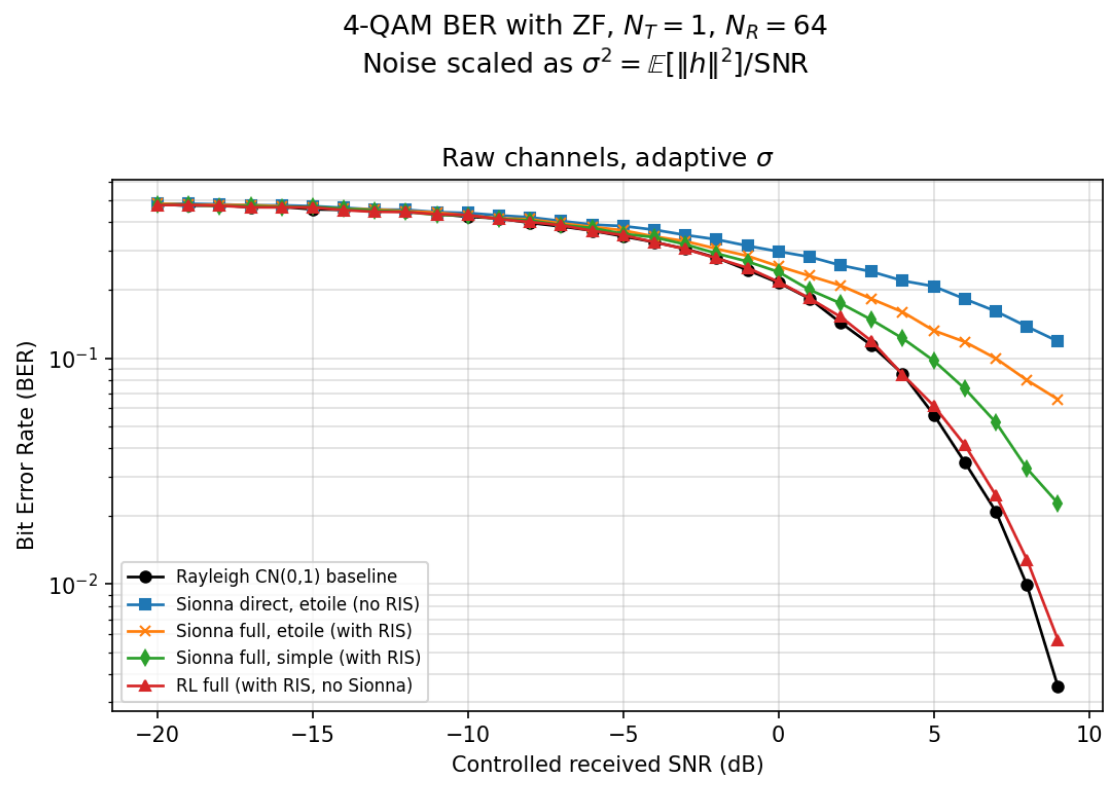
\includegraphics[width = 0.65\textwidth]{Figures/BER_normalized_channels_sionna.png}
            % \caption{\centering \parbox{0.6\textwidth}{Comparison of benchmarks for selecting the optimal configuration for the RIS.}}
        % \end{figure}
        
    \end{frame}    


    %------------------------------------------------
    % Bibliography
    %------------------------------------------------

    \begin{frame}
        \frametitle{Scientific contributions}
        \bibliographystyle{IEEEtran} 
        \bibliography{bibtex}  
        \end{frame}

    %------------------------------------------------

    \section{Future Perspectives}

    %------------------------------------------------

    \begin{frame}
        \frametitle{Future Perspectives}
            \begin{itemize}
            \item \textit{Mobile user scenario:} \begin{itemize}
                \item Validate the performance of our proposed approach on the generated channels with the Sionna framework.
                \item Handle user mobility and time-varying channels.
                \item Do a a real-world experiment with RIS prototypes
            \end{itemize}
            \pause
            \item \textit{Multi-user extension:} Scale the study to multi-user scenarios.
            \end{itemize}
    \end{frame}

    %------------------------------------------------
    % End page
    %------------------------------------------------

    \title{\textcolor{purple}{Thank you! Questions?}}
    \begin{frame}{}
        \maketitle
    \end{frame}

    %------------------------------------------------
    % Appendix
    %------------------------------------------------

    \begin{frame}
        \frametitle{Euclidean distance}
        \begin{equation}
            \mathbf{p}(\boldsymbol{\Phi}(\mathbf H) = \boldsymbol{\Phi}_k| \mathbf Y_{1}^{\mathrm L_p},\boldsymbol{\Psi}_{1}^{\mathrm L_p}) \propto
            \mathbf{p}(\boldsymbol{\Phi}(\mathbf H) = \boldsymbol{\Phi}_k| \mathbf Y_{1}^{\mathrm L_p-1},\boldsymbol{\Psi}_{1}^{\mathrm L_p-1})  
            \cdot\sum_{\mathbf H_{\mathrm l} / \mathbf S_{\mathrm T}(\mathbf H_{\mathrm l})[k] = 1}  
            \frac{1}{(\mathbf X(\mathbf H_{\mathrm l})[\mathrm L_p]-\mathbf Y_{\mathrm L_p})^2}
        \end{equation}
    \end{frame}

    %------------------------------------------------

    \begin{frame}
        \frametitle{Stochastic shortest path problem}
        \centering
        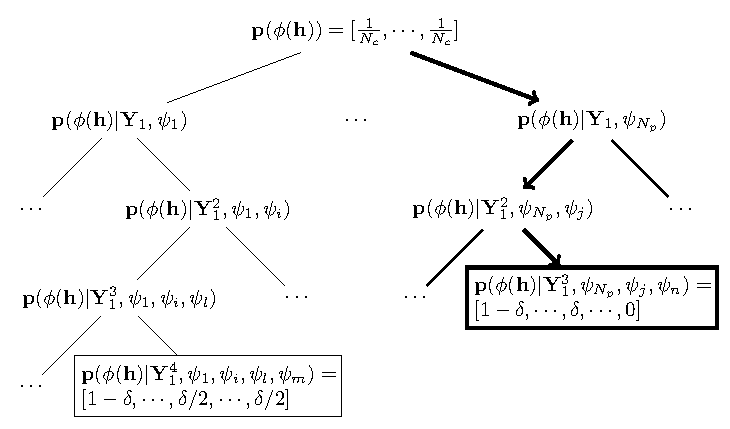
\includegraphics[width = 0.7\textwidth]{Figures/Tree_short.pdf}
    \end{frame}

    %------------------------------------------------

    \begin{frame}
        \frametitle{Stochastic shortest path problem}
        \centering
        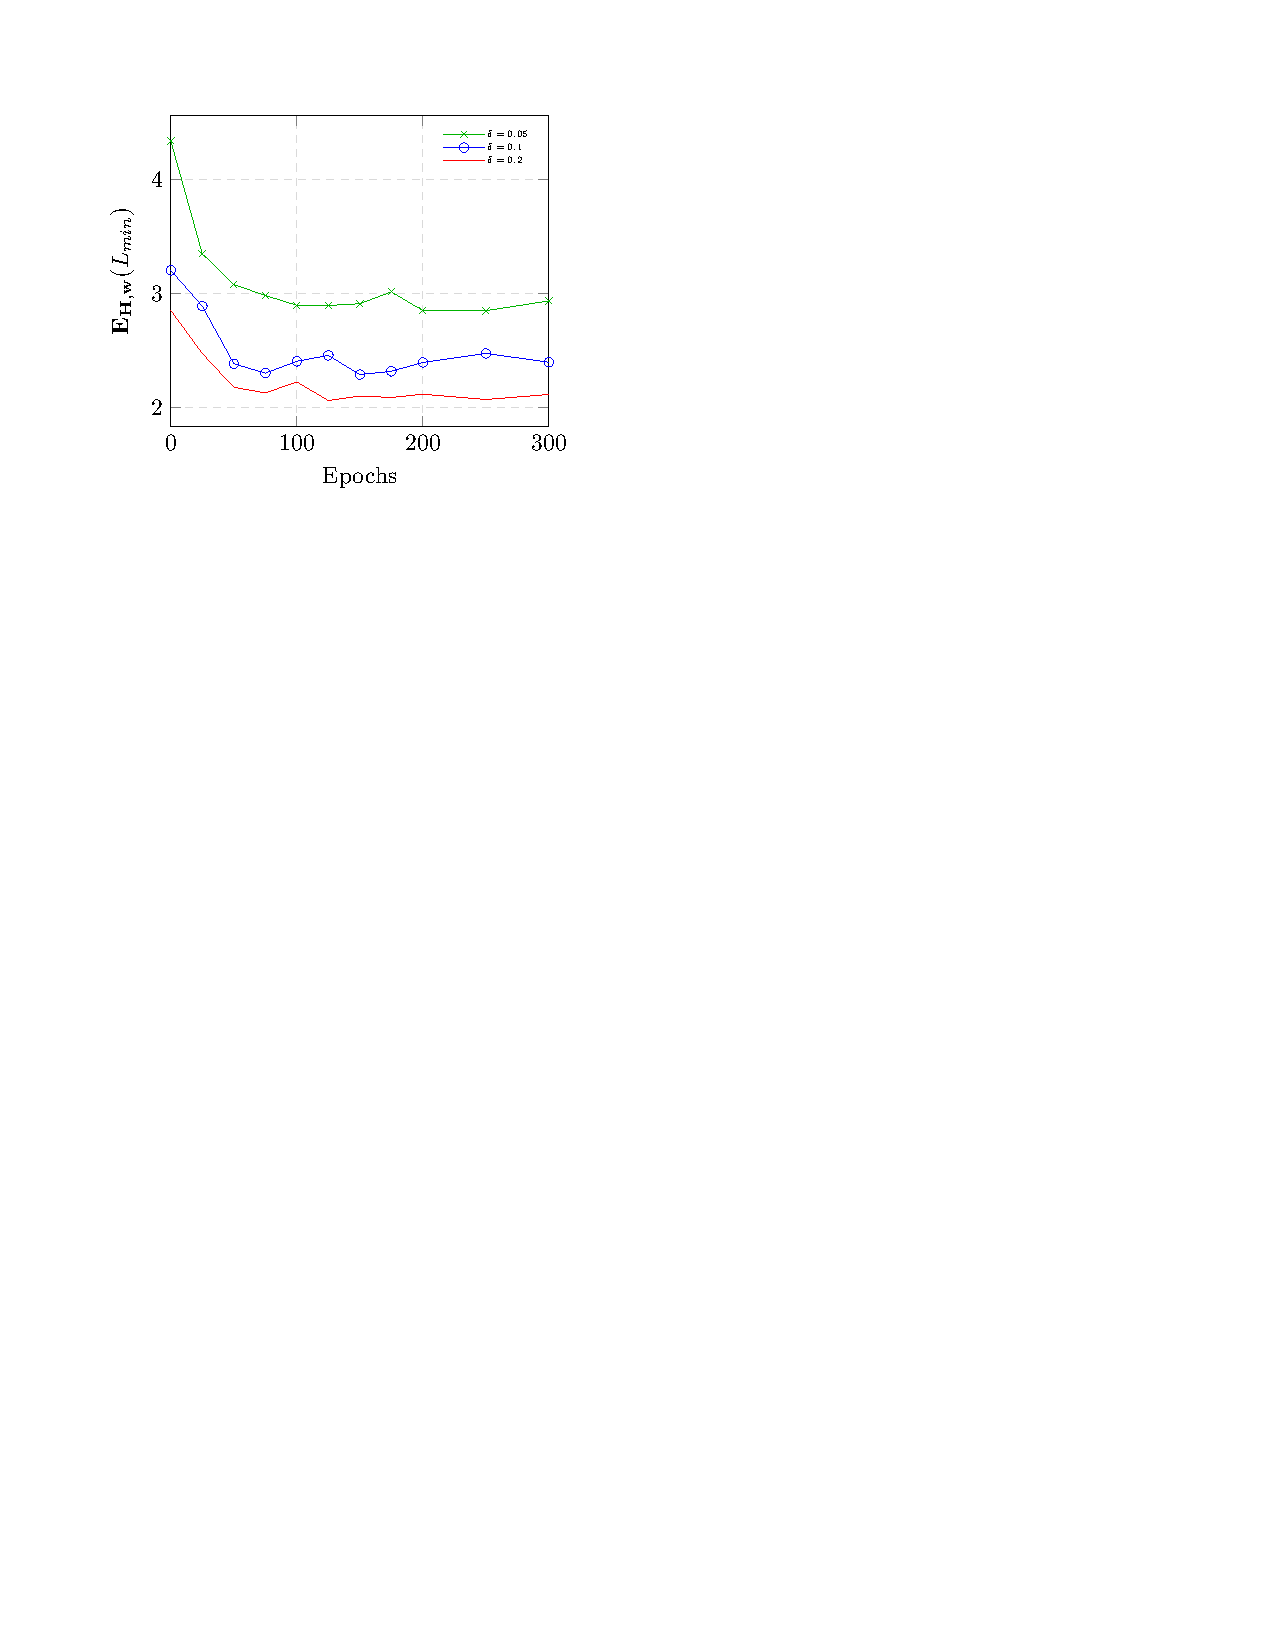
\includegraphics[width = 0.6\textwidth]{Figures/avg_len_path_delta.pdf}
    \end{frame}
    
    %------------------------------------------------

    \begin{frame}
        \frametitle{Q-Learning algorithm}
        \centering
        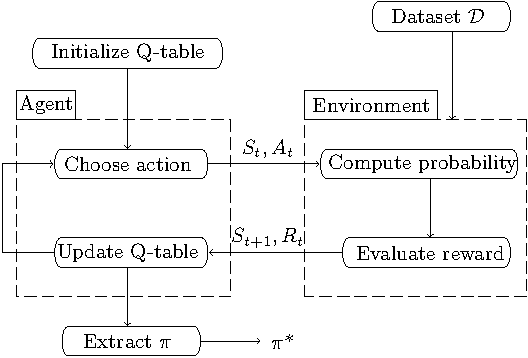
\includegraphics[width = 0.6\textwidth]{Figures/agent_env2.pdf}
    \end{frame}

    
    %------------------------------------------------

    \begin{frame}
        \frametitle{Proposed approach : Reinforcement Learning}
        \framesubtitle{Stochastic shortest path problem}
        \centering
        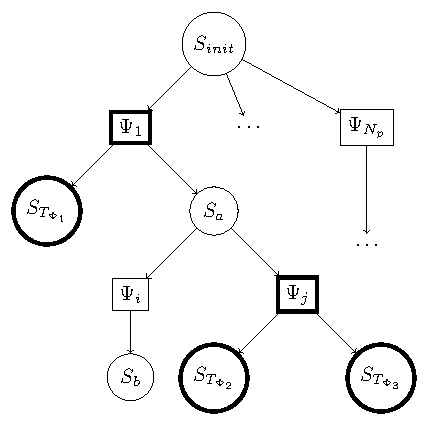
\includegraphics[width = 0.4\textwidth]{Figures/Graph.pdf}
    \end{frame}
    
    %------------------------------------------------

    \begin{frame}
        \frametitle{Sionna - Scene view}
        \framesubtitle{The area around the Arc de Triomphe in Paris}
        \centering
        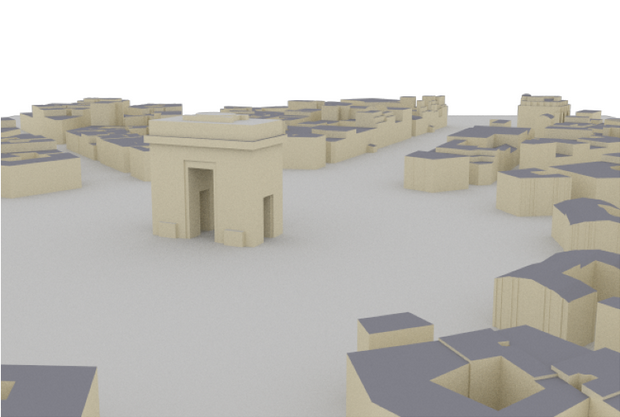
\includegraphics[width = 0.5\textwidth]{Figures/scene_etoile.PNG}
    \end{frame}

    %------------------------------------------------

    \begin{frame}
        \frametitle{Sionna - Scene view}
        \framesubtitle{Simple floor-wall scenario}

        \centering
        \begin{tikzpicture}
            \node[anchor=south west, inner sep=0] (img) at (0,0)
            {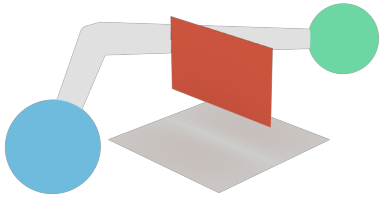
\includegraphics[width=0.55\textwidth]{Figures/scene_visualization_3D.png}};

            % Labels
            \node[blue!70!black, font=\bfseries\large] at (-0.45,2.35) {BS};
            \node[red!70!black, font=\bfseries\large] at (1.1,4.8) {RIS};
            \node[green!50!black, font=\bfseries\large] at (8.8,4.80) {UE};

            % Optional arrows
            \draw[->, blue!70!black, thick] (-0.55,2.07) -- (0.35,1.8);
            \draw[->, red!70!black, thick] (1.35,4.6) -- (1.8,3.65);
            \draw[->, green!50!black, thick] (9.0,4.5) -- (8.05,3.95);
        \end{tikzpicture}

        \vspace{0.25cm}
        {\scriptsize Visualization of the simulated scenario with a BS (64 antennas), \\
        \centering {a RIS (1D 100 elements), and a UE (a single antenna).}}
    \end{frame}

    \begin{frame}
        \begin{align*}
            \text{a}_{\text{i}}^{\text{b}} &= \text{a}_{\text{i}} e^{-\text{j} 2\pi \text{f} \tau_{\text{i}}} \\
            \text{H}(f) &= \sum_{\text{i}}^{}\text{a}_{\text{i}} e^{-\text{j} 2\pi \text{f} \tau_{\text{i}}} \\
            g_{\text{i},\text{j}} &= \frac{1}{|C|} \int_{C_{\text{i},\text{j}}}{} |h(s)|^2 ds \\ 
            \text{RSS}_{\text{i},\text{j}} &= \text{P}_\text{tx} . \text{g}_{\text{i},\text{j}} \\
            \text{N}_{0} &= \text{k} . \text{T} . \text{B} \,[\text{W/Hz}] \\
            \sigma^2 &= 10 \log_{10} (\text{N}_{0}) \,[\text{W}] \\
            \text{SNR} &= 10 \log_{10} (\frac{\text{P}_\text{tx} \|h\|^2}{\sigma^{2}}) \\ 
            \tau_{\text{i}} &= \text{a}_{\text{i}} \\
            \sigma^2 &= -174 + 10 \log_{10} \text{B} \,[\text{dBm}] = -94\,[\text{dBm}]\\
            \text{P}_\text{dBm} &= 30 + 10 \log_{10} \text{P}_{\text{W}}
        \end{align*}
    \end{frame}

    \begin{frame}
        \begin{align*}
        \mathrm{SINR}_{i,j}^{k}
        &=
        \frac{\mathrm{RSS}_{i,j}^{k}}
        {N_{0} + \sum_{k' \ne k} \mathrm{RSS}_{i,j}^{k'}} \\
        \mathrm{R} &= (\mathrm{H}^{\text{H}}\mathrm{H})^{-1}\mathrm{H}^{\text{H}} \\
        \mathrm{y} &=\mathrm{H}\mathrm{x} + \mathrm{W} \\
        \mathrm{R}\mathrm{y} &= \mathrm{x} + \mathrm{R}\mathrm{W} \\ 
        \mathrm{E}_{\mathrm{x}_\text{tx}} &= \sum \left|\mathrm{x}_{\text{tx}}\right|^{2}\\
        \mathrm{E}_{\hat{\mathrm{x}}} &= \sum \left|\hat{\mathrm{x}}\right|^{2}\\
        \mathrm{E}_{\mathrm{y}_{\text{mrc}}} &= \sum \left|\mathrm{y}_{\text{mrc}}\right|^{2}\\
        &= {\left\lVert \mathrm{H} \right\rVert}^{2} \mathrm{E_s} + \sigma_w^2\\
        \mathrm{y}_{\text{mrc}} &= \frac{\mathrm{H}^{\mathrm{H}}\mathrm{y}}{\left\lVert \mathrm{H} \right\rVert}\\
        &= \left\lVert \mathrm{H} \right\rVert \mathrm{x}_\text{tx} + \frac{\mathrm{H}^{\mathrm{H}}\mathrm{W}}{\left\lVert \mathrm{H} \right\rVert}
        \end{align*}
    \end{frame}

    \begin{frame}
        \begin{align*}
            \frac{\mathrm{E}_{\hat{\mathrm{x}}}}{\mathrm{E}_{\mathrm{x}_\text{tx}}} \\
            \left\lVert \mathrm{H} \right\rVert \mathrm{E}_{s} \ll \sigma_w^2\\
            \left\lVert \mathrm{H} \right\rVert \mathrm{E}_{s} \gg \sigma_w^2\\
            \sigma_w^2 &= \frac{{\left\lVert \mathrm{H} \right\rVert}^{2} \mathrm{E}_{s}}{\text{SNR}_{\text{linear}}} \\
            \sigma_w^2 &= \frac{\mathrm{E}_{s}}{\text{SNR}_{\text{linear}}} \\
            \text{SNR}_{\text{real}} &= \frac{{\left\lVert \mathrm{H} \right\rVert}^{2} \mathrm{E}_{s}}{\sigma_w^2} \\
            &= \frac{{\left\lVert \mathrm{H} \right\rVert}^{2} \mathrm{E}_{s}}{\frac{\mathrm{E}_{s}}{\text{SNR}_{\text{linear}}}} \\
            &= {\left\lVert \mathrm{H} \right\rVert}^{2} \text{SNR}_{\text{linear}}
        \end{align*}
    \end{frame}

    \begin{frame}
        \begin{align*}
            \mathrm{SNR}_{\text{real}} &= \frac{P_{\mathrm{tx}} \left\|H\right\|^2}{\sigma_{W}^2} \\
            \Longrightarrow \quad
            P_{\mathrm{tx}} &= \frac{\mathrm{SNR}_{\text{real}}\,\sigma_{W}^2}{\left\|H\right\|^2} \\
            x &= 7 \pi sin(\Phi) \\
            y_j &= r_j + \gamma Q(\Phi_{j+1}, \arg\max_{a'} Q(\Phi_{j+1},a';\theta);\theta^-) \\
            \delta_t &= r_t + \gamma (1 - d_t) V_{t+1} - V_{t} \\
            A_t &= \delta_t + \gamma \lambda(1 - e_t) A_{t+1} \\
            R_t &= A_t + V_t \\
            r_t(\theta) &= \frac{\pi_\theta(a_t \mid s_t)}{\pi_{\theta_{\mathrm{old}}}(a_t \mid s_t)} 
        \end{align*}
    \end{frame}

    \begin{frame}
        \begin{align*}
            L_t^{\mathrm{CLIP}}(\theta) &= \min\left(r_t(\theta)A_t,\operatorname{clip}\left(r_t(\theta),1-\epsilon,1+\epsilon\right)A_t\right) \\
            L_{\mathrm{actor}} &= -\mathbb{E}_t\left[\min\left(r_t(\theta)A_t,\operatorname{clip}\left(r_t(\theta),1-\epsilon,1+\epsilon\right)A_t\right)\right] \\
            L_{\mathrm{critic}} &= \frac{1}{2}\mathbb{E}_t\left[\left(V_t-R_t\right)^2\right] \\
            L_{\mathrm{critic}} &= \frac{1}{2}\mathbb{E}_t\left[\left(V_\Phi(s_t)-R_t\right)^2\right] \\
            H(\pi_\theta) &= -\mathbb{E}_t\left[\sum_a\pi_\theta(a\mid s_t)\log\pi_\theta(a\mid s_t)\right] \\
            L_{\mathrm{total}} &= L_{\mathrm{actor}} + c_v L_{\mathrm{critic}} + c_e L_{\mathrm{entropy}}
        \end{align*}
    \end{frame}

    \begin{frame}{Proximal Policy Optimization: Approximate KL Divergence}

        \textbf{True KL divergence:}
        \begin{align*}
        D_{KL}\left(\pi_{\text{old}} \,\|\, \pi_\theta\right) &= \mathbb{E}_t\left[\log \frac{\pi_{\text{old}}(a_t \mid s_t)}{\pi_\theta(a_t \mid s_t)}\right]
        \end{align*}

        \textbf{Estimators} (with $r_t(\theta) = \dfrac{\pi_\theta(a_t\mid s_t)}{\pi_{\text{old}}(a_t\mid s_t)}$, $\log r_t = \log\pi_\theta - \log\pi_{\text{old}}$):

        \begin{align*}
        k_1 &= -\log r_t \\[4pt]
        k_2 &= \tfrac{1}{2}\left(\log r_t\right)^2 \\[4pt]
        k_3 &= \left(r_t - 1\right) - \log r_t
        \end{align*}
        \vspace{-3mm}
        \textbf{Early stopping rule:}
        \begin{align*}
        \text{if } \; \hat{D}_{KL} &= \frac{1}{N}\sum_{t=1}^{N} k_3^{(t)} \;>\; \delta_{\text{target}} \quad \Rightarrow \quad \text{stop epoch updates}
        \end{align*}

    \end{frame}

    \begin{frame}
        $$p(Y_{1:S}\mid c);=;\int p(Y_{1:S}\mid h,\varphi_{1:S});p(h\mid c);dh .$$
        $$\text{posterior}(c);\propto;\text{prior}(c);\cdot;\mathcal{L}(c)\qquad(\text{then}+10^{-8}\text{ and normalise to sum }1)$$
    \end{frame}
%     %---------------------Poster---------------------------
%     \begin{frame}
%         \begin{itemize}
%             \item 5G \& 6G rely on Milimiter waves (mmWaves) for a higher coverage;
%             \item mmWaves suffer from fading environments;
%             \item RIS is a promising solution with low power consumption;
%             \item Channel estimation is challenging. Focus on blind methods where the channel $\mathbf H$ is unkown.
%             \item Number of users ($\mathrm N_{\text{UE}}$): 1;
%             \item Number of antennas ($\mathrm N_{\text{BS}}$): 64;
%             \item Number of RIS elements ($\mathrm N_{\text{RIS}}$): 100;
%             \item The direct link $\mathbf{h}_{D}$ is blocked.
%             \end{itemize}
%     \end{frame}

%     %------------------------------------------------

%     \begin{frame}
%         \onslide We consider half-wave spaced uniform linear arrays :
%         \vspace{3mm} \\
%         \begin{equation*}
%             \begin{split}   
%                 \bold{H}_{BS} &=  \mathbf{a}_{\mathrm N_{\text{RIS}}}(\Phi_{1}) \mathbf{a}_{\mathrm N_{\text{BS}}}^H(\Phi_{2}) \\
%                 \bold{h}_{UE} &=  \mathbf{a}_{1}(\Phi_{3}) \mathbf{a}_{\mathrm N_{\text{RIS}}}^H(\Phi_{4}) 
%             \end{split}
%         \end{equation*}
%         \onslide where the steering vector is : 
%         \vspace{3mm}
%         \begin{equation*}
%             \mathbf{a}_{\mathrm N_{\text{RIS}}}(\Phi) = [1,e^{j\pi \sin (\Phi)},\ldots, e^{j\pi (\mathrm N_{\text{RIS}}-1) \sin (\Phi)}]^T
%         \end{equation*}
%         \vspace{3mm}
%         The signal received at the BS is:
%         \begin{equation*}
%             \mathbf y = \sqrt{P}\mathbf{H}_{BS} \boldsymbol{\Theta} \mathbf{h}_{UE} s + w
%         \end{equation*}
%         \vspace{3mm}
%         The full channel between the UE and the BS is:\\
%         Achievable rate between the UE and the BS:
%     \end{frame}

%     %------------------------------------------------

%     \begin{frame}
%         \begin{equation*}
%             \mathrm{R} 
%             = 
%             \max_{i \in \llbracket N_c \rrbracket} 
%             \left [
%                 \log_2 \left ( 1+\frac{P \|\bold{H}_{BS} \text{diag}({\Phi_{i}}) \mathbf{h}_{UE}\|_2^2 }{\sigma_w^2} \right )
%             \right ]
%         \end{equation*}
%     \end{frame}

%     \begin{frame}
%         \begin{equation*}
%             \mathbf h(\boldsymbol{\Phi}) = \bold{H}_{BS} \boldsymbol{\Theta} \mathbf{h}_{UE} \\
%             \mathrm L_{\text{min}} = -\sum_{t=0}^{\infty} R_t
%         \end{equation*}  \\
%         Let $\boldsymbol{\Phi}$ be the codebook for communication and $\boldsymbol{\Psi}$ the codebook used for pilots. \\
%         We define the class $\boldsymbol{\Phi}(\mathbf H)$ : 
%         \begin{equation*}
%             \boldsymbol{\Phi}(\mathbf H) = \{i \in \llbracket N_c \rrbracket : \Phi_{i} = \argmax_{i \in \llbracket N_c \rrbracket} \!\ (||\bold{h}(\boldsymbol{\Phi_{i}})||_2^2)\}.
%         \end{equation*}
%     \end{frame}
%     \begin{frame}
%         \begin{block}{Objective}
%             For $\delta \in [0;1]$, we want to find the optimal configuration $\Phi_{opt} \in \boldsymbol{\Phi}$ while minimizing the number of required pilots $\Psi \in \boldsymbol{\Psi}$. Thus, we need to find $\mathrm L_{min}$ st. the probability of correct classification respects a fixed degree of precision $\delta$ :
%             \begin{equation*}
%                 \mathrm L_{\min} = \min \{\mathrm L_p : \| p(\boldsymbol{\Phi}(\mathbf H) | Y_1^{\mathrm L_p},\boldsymbol{\Psi}_1^{\mathrm L_p}) \|\infty >1-\delta\}
%             \end{equation*}
%         \end{block}
%         \raggedright $\mathbf S_{T_{Real}} = [\mathbf S_{T}(\mathbf H_1),\ldots,\mathbf S_{T}(\mathbf H_{N_{Dataset}})]$, where $\mathbf{S}_T(\mathbf H_k) = [0 \cdots 0 \underset{\substack{\downarrow \\ \text{\it $c^{*}$}}}{1} 0  \cdots 0 ] $,
%         $c^{*} = \argmax_{c \in [1;N_c]} ||\bold{h}(\Phi_c)||_2^2)$.
%     \end{frame}
\end{document} 